%% Šablona pro psaní závěrečných prací FBMI ČVUT
% Upraveno na základě požadavků na závěrečné práce schválených dne 24.2.2020.
%
% Vytvořeno ve spolupráci členů BRAIN Teamu.
% 
% Šablonu pro vás upravil/a:    Ing. Václava Piorecká, Ph.D.
% Kontakt:                      vaclava.piorecka@fbmi.cvut.cz
%
% % % % % % % % % % % % % % % % % % % % % % % % % % % % % % 
%
% 		Upravená verze pro xeLaTeX by Marek Sokol :)			
%  
% % % % % % % % % % % % % % % % % % % % % % % % % % % % % % 

% arara: xelatex: { shell : yes }
%% arara: biber
%% arara: xelatex: { shell : yes }
%% arara: xelatex: { shell : yes }

\documentclass[a4paper,12pt]{article}   % Definice - velikost dokumentu, základní velikost písma, typ
\usepackage[a4paper, top=2.5cm, left=3.5cm, right=2.5cm, bottom=2.5cm]{geometry}		% nastavení okrajů

%% Přidání balíčků podporujících různé funkcionality - ZÁKLADNÍ
\usepackage{amsmath,float}				% balíček pro matiku
\usepackage[dvipsnames]{xcolor}
\usepackage{color}
\usepackage{footnote}					% poznámka pod čarou
\usepackage{url}						% url odkazy
\DeclareUrlCommand\url{\def\UrlLeft{<}\def\UrlRight{>} \urlstyle{same}}   % nastavení URL odkazů pro podle normy ČSN ISO 690

\usepackage{float}						% plovoucí prostředí
%\usepackage[utf8]{inputenc}			% kódování (v tomto případě useless protože používáme unicode engine)
\usepackage[czech]{babel}				% čeština
\usepackage{enumitem}      			    % seznamy 
\usepackage{xevlna}						%
\usepackage{subcaption}					%
\usepackage{pdfpages}					%
\usepackage{amsfonts}      				% množiny Z,R,N dvojitě
\usepackage{amssymb}      				% znaky úhlu a tak
\usepackage{graphicx}					%
\usepackage{textgreek}					%
\usepackage{setspace}					%
\usepackage{multicol}					% tabulka, slučování sloupců
\usepackage{multirow}                   % tabulka, slučování řádků
\usepackage{fancyhdr}					% záhlaví a zápatí stránky
\usepackage{chngcntr}                   % číslování (číslování rovnic, obrázků dle kapitol)
\usepackage{array}                      % rozšíření práce s tabulkami
\usepackage{helvet}                     % předefinuje \sfdefault to uhv (pro úvodní stránku)
\usepackage[flushleft]{threeparttable}  % prostředí pro tabulky - přidává vysvětlující poznámky pod tabulku

\usepackage{tikz}
\usetikzlibrary{shapes.geometric, arrows, fit}
\tikzstyle{startstop} = [rectangle, minimum width=3cm, minimum height=1cm,text centered, draw=white, fill=white]
\tikzstyle{io} = [trapezium, trapezium left angle=70, trapezium right angle=110, minimum width=3cm, minimum height=1cm, text centered, draw=black, fill=white]
\tikzstyle{process} = [rectangle, minimum width=3cm, minimum height=1cm, text centered, draw=black, fill=white]
\tikzstyle{decision} = [diamond, minimum width=3cm, minimum height=1cm, text centered, draw=black, fill=white]
\tikzstyle{invisible} = [rectangle, text=white]
\tikzstyle{arrow} = [thick,->,>=stealth]

% Následující balíčky řeší citace v dokumentu. 
\usepackage{csquotes}   
\usepackage{expl3}                    
\usepackage[style=iso-numeric]{biblatex}
\addbibresource{biblio.bib}             % zdrojový soubor s citacemi

\usepackage{siunitx}					%
%% Přidání balíčků podporujících různé funkcionality - VOLITELNÉ, DOPLŇKOVÉ
% Existuje celá řada dalších
%\usepackage[]{algorithm2e}				    % balíček pro pseudokód
%\usepackage{ifthen}                        % pro algoritmy if else
%\usepackage{paralist}                      % Rozšířená možnost pro seznamy. Větší škála a možnosti jak seznamy dělat automaticky. 
%\usepackage{courier}
\usepackage{fontspec}                       % nastavení specifických fontů
\setmainfont{Times New Roman}
\setsansfont{Arial}
\setmonofont[Scale=0.9]{Courier New}
%\usepackage{icomma}      				    % není mezera za desetinnou čárkou
% \usepackage[titletoc,title]{appendix}     % automatické vytvoření příloh

%% Přidání speciálních příkazů 
\newcommand{\TextUnderscore}{\rule{.4em}{.4pt}}
\newcommand{\at}{\makeatletter @\makeatother}           % Vytiskne zavináč - \at
\newcommand{\degree}[1][]{\ensuremath{{#1}^\circ}}      % Vytiskne stupeň - \degree
\newcolumntype{C}[1]{>{\centering\let\newline\\\arraybackslash\hspace{0pt}}m{#1}}	% zarovnání v tabulce, vycentrování, potřebuje \usepackage{array}
\addto\captionsczech{\renewcommand{\figurename}{Obr.}}		%

% Zalamování slov na konci věty - napodobení justify jako MS-Word
%\tolerance=1
%\emergencystretch=\maxdimen
%\hyphenpenalty=10000
%\hbadness=10000
%\sloppy

%% Ostatní definice a nastavení
\clubpenalty 10000		% penalizace sirotků, sirotek: poslední řádek odstavce je na nové stránce
\widowpenalty 10000		% penalizace vdov, vdova: první řádek nového odstavce je na konci stránky

\DeclareGraphicsExtensions{.pdf,.png,.jpg}	    % nahrávání obrázků, rozšíření
\graphicspath{{assets/}} 				        % umístění obrázků

\counterwithin{figure}{section}         % číslování obrázků dle sekcí/kapitol
\counterwithin{table}{section}          % číslování tabulek dle sekcí/kapitol
\numberwithin{equation}{section}        % číslování rovnic dle sekcí/kapitol

\setlength{\parskip}{6pt}                   % odsazení mezi odstavci
\setlength{\parindent}{0.75cm}              % odsazení odstavců od okraje
\renewcommand{\baselinestretch}{1.20}	    % řádkování 1,2 - odpovídá pevnému řádkování 17 bodů

\usepackage{tocloft}                    % Nastaví tučné zvýraznění sekcí v obsahu
\renewcommand{\cftsecleader}{\cftdotfill{\cftdotsep}}   % přidá vodící linku do obsahu u sekcí

%% Ostatní neimplementované, pouze návod jak případně doplnit
% Vytvořit seznam použitých algoritmů a přejmenování názvu objektu na Algoritmus.
\usepackage{listings}
\usepackage[algosection,vlined,linesnumbered]{algorithm2e}
\SetAlgorithmName{Algoritmus}{algorithm}{Seznam algoritmů}
\SetKwInput{KwIn}{Vstup}%
\SetKwInput{KwOut}{Výstup}%
% // TODO: Turn on referencing
% \usepackage{hyperref}%
   
%% Deklarace názvů - přepsat dle autora
\newcommand{\autor}{Marek Sokol}
\newcommand{\vedouci}{Mgr. Ksenia Sedova, Ph.D.}
\newcommand{\nazev}{Zpracování a analýza záznamu srdeční aktivity}
\newcommand{\nazevENG}{Heart activity record processing and analysis}
\newcommand{\typ}{Bakalářská práce}
\newcommand{\rok}{2021}
% Pro program a obor jsou instrukce zde: http://www.fbmi.cvut.cz/fakulta/uredni-deska 
% Nově akreditované mají pouze studijní programy
\newcommand{\program}{Biomedicínská a klinická technika}
\newcommand{\obor}{Biomedicínský technik}       % u nových akreditací vypustit

%% Vlastní začátek dokumentu
\begin{document}

\pagestyle{empty}

\begin{titlepage}
	\begin{center}
		\begin{figure}[!h]
			\centering
			\includegraphics[width=0.2\textwidth]{symbol_cvut_konturova_verze}
		\end{figure}
		\textsf{\large{\textbf{ČESKÉ VYSOKÉ UČENÍ TECHNICKÉ V PRAZE}}}\\
		%\vspace{0pt}   		
		{\color{NavyBlue}\makebox[\linewidth]{\rule{\textwidth}{0.4mm}}}
		%{\color{NavyBlue}\hrule }  	    \vspace{6pt}
		\textsf{\normalsize{\textbf{FAKULTA BIOMEDICÍNSKÉHO INŽENÝRSVÍ}}}\\
		\textsf{\textbf{Katedra biomedicínské techniky}}\\

		\vfill

		\textsf{\Large{\textbf{\nazev}}}\\
		\vspace{24pt}
		\textsf{\Large{\textbf{\nazevENG}}}\\
		\vspace{24pt}
		\textsf{\typ}\\
		\vfill
	\end{center}
	\textsf{Studijní program: \program} \\
	\textsf{Studijní obor: \obor} \\ % u nových akreditací zakomentovat či smazat tento řádek
	\\
	\textsf{Vedoucí práce: \vedouci}\\

	\begin{center}
		\textsf{\textbf{\autor}} \\ [0.5cm]

		{\color{NavyBlue}\makebox[\linewidth]{\rule{\textwidth}{0.4mm}}}

		\textsf{\textbf{Kladno \rok}}
	\end{center}

	\clearpage

\end{titlepage}

% Vloženi kopie zadaní v pdf
\includepdf[pages=-, trim=1mm 1mm 6mm 1mm, clip]{assignment/assignment_colored}

\null\vfill
\section*{Prohlášení}
% \hspace ruší odsazení odstavce - v šabloně u prohlášení odstavce odsazené nejsou. 
Prohlašuji, že jsem bakalářskou práci s názvem \uv{\nazev} vypracoval/a samostatně a~použil/a k~tomu úplný výčet citací použitých pramenů, které uvádím v seznamu přiloženém k~bakalářské práci.

\hspace{-0.75cm}Nemám závažný důvod proti užití tohoto školního díla ve smyslu \S 60 Zákona č.121/2000~Sb., o~právu autorském, o~právech souvisejících s právem autorským a~o~změně některých zákonů (autorský zákon), ve znění pozdějších předpisů.

\vspace{1em}

\hspace{-0.75cm}V Kladně dne \ldots \ldots \ldots \hfill \ldots \ldots \ldots \ldots \ldots \ldots \ldots \ldots \ldots \ldots

\hspace{10cm} \textbf{\autor}

\clearpage

\null\vfill
\section*{Poděkování}
% Mé poděkováni patři též XXXXXXXX za spolupráci při získávání údajů pro výzkumnou část práce.
Rád bych poděkoval vedoucí své bakalářské práce, Mgr. Ksenii Sedové, Ph.D. za
odborné vedení práce, za pomoc, vstřícnost a rady při zpracování této práce.
Dále bych rád poděkoval panu Ing et Ing. Janu Hejdovi, Ph.D. za všestrannou
pomoc, množství cenných a inspirativních rad, podnětů, doporučení a čas, který
mi věnoval při řešení dané problematiky. V neposlední řadě děkuji své rodině a
všem přátelům, kteří mě při vytváření této práce podpořili.

\clearpage


\null\vfill
\section*{ABSTRAKT}
\subsection*{\nazev:}
Bakalářská práce se věnuje návrhu a realizaci softwarového řešení pro hodnocení
srdeční aktivity v programovém prostředí MATLAB a Python. Hlavním cílem je
navrhnout adaptivní algoritmus v prostředí MATLAB, který bude schopný realizovat
offline analýzu na naměřeném EKG signálu zatíženého artefakty pomocí Poincarého
grafu. Pro hodnocení zpracovaného záznamu byla vybraná analýza v časové oblasti,
konkrétně variabilita srdeční frekvence a z ní vycházející parametry. Dalším
cílem práce je navrhnout a realizovat řešení s GUI pro online hodnocení srdeční
aktivity v prostředí Python. K testování navrženého řešení byly použity
krátkodobé záznamy naměřené celkem u 5 probandů. Během měření byli probandi
nejdříve v klidu a následně byl každý z nich vystaven situaci stimulující
kognitivní zátěž. Každý z probandů byl během měření monitorován Holterem neboli
přenosným elektrokardiografem. Výsledkem práce je sada skriptů implementovaných
v prostředí MATLAB schopných offline adaptivně zpracovat EKG a zobrazit grafy
parametrů prokazujících korelaci kognitivní zátěže s variabilitou srdečního
rytmu v závislosti na čase. Byla naprogramována multiplatformní Python GUI
aplikace rozšiřující výstup v rámci online měření. 


\subsection*{Klíčová slova}
EKG (Elektrokardiogram), zpracování EKG, detekce EKG komponentů, EKG analýza, HRV analýza, HRV parametry, MATLAB, Python
\clearpage


\null\vfill
\section*{ABSTRACT}
\subsection*{\nazevENG:}
\begin{otherlanguage}{english}
This bachelor's work describes designing and implementing a software
solution to evaluate cardiac activity in MATLAB and Python
software environments. The main goal is to design an adaptive algorithm in the
MATLAB environment, that will perform offline analysis of the
measured ECG signal with artefact. The nonlinear geometric method of the
Poincaré graph was chosen for the analysis of the processed record, which
evaluates the variability of the heart rate. Another goal of this work is to
design and implement a solution with a GUI for the online evaluation of cardiac
activity in the Python environment. For testing the proposed solution,
short-term records measured in a total of 5 probands were used. During the
measurement, the probands were first at rest, and then each of them was exposed
to a situation that stimulates cognitive stress. Each of the probands was
monitored during the measurement by Holter, a portable electrocardiogram. The
result of the work is a MATLAB application capable of adaptively processing the
measured ECG recordings and displaying graphs of parameters demonstrating the
correlation of cognitive load with HRV over time. A
multiplatform Python GUI application was programmed, extending the output within
the online measurement and processing of ECG. 
\end{otherlanguage}
\subsection*{Key words}
ECG (Electrocardiogram), ECG processing, detection of ECG components, ECG analysis, HRV analysis, HRV parameters, MATLAB, Python
\clearpage

\pagestyle{plain}	% Číslování stránek začíná odsud

\tableofcontents			% Vloží obsah

\clearpage

\section*{Seznam symbolů a zkratek} %sekce = nadpis, s * není v obsahu
\addcontentsline{toc}{section}{Seznam symbolů zkratek}
\subsection*{Seznam symbolů}

\begin{table}[h]
	\label{tab:symboly}
	\catcode`\-=12          % Tento řádek je tam kvůli použití cline pro czech babel. Jinak to bere pomlčku jako znak a nevnímá ji jako rozsah. 
	\begin{center}
		\begin{tabular}{p{2.5cm}p{2.5cm}p{9.25cm}}
			\noalign{\hrule height 2pt}
			Symbol                 & Jednotka & Význam    \\
			\noalign{\hrule height 2pt}
			$|H_i(\widetilde{w})|$ & -        & Magnituda \\
			% $\delta_1$             &     &                                            \\
			% $\delta_2$             &     &                                            \\
			% $\omega_d$             &     &                                            \\
			% $\omega_h$             &     &                                            \\
			% $y_n$                  &     &                                            \\
			% $H(z)$                 &     &                                            \\
			% $h_n$                  &     &                                            \\
			% $G(w)$                 &     &                                            \\
			% $L_i$                  &     &                                            \\
			% $Ki$                   &     &                                            \\
			% $A$                    &     &                                            \\
			% $p_i$ & & \\
			% $n_i$ & & \\
			% $\Phi_i$ & & \\
			% $\Psi_i$ & & \\
			% $w[n]$ & & \\
			% $I_0$ & & \\
			% $\Beta$ & & \\
			% $\alfa$ & & \\
			% $d[n]$                 & mV          & Diferencovaný signál              \\
			% $f[n]$                 & mV          & Původní signál                    \\
			% $Ww$                   & s           & Délka pevného okna (Window width) \\
			% $Bc[n]$                & mV          & Zpětně kumulovaný signál          \\
			% $RR$                   & s           & Délka R-R intervalu               \\
			% $\overrightarrow{RR}$ & & \\
			% $Th_amp$ & & \\
			% $R_m$ & & \\
			% $Th_RR$ & & \\
			% $dRRs$ & & \\
			% $Th1$ & & \\
			% $dRR$ & & \\
			% $mRRs$ & & \\
			% $Th2$ & & \\
			% $mRR$ & & \\
			% $S11$ & & \\
			% $S12$ & & \\
			% $S21$ & & \\
			% $S22$ & & \\
			% $x1$ & & \\
			% $x2$ & & \\
			% $a$ & & \\
			% $b$ & & \\
			% $x$ & & \\
			% $y$ & & \\
			% $X$ & & \\
			% $Y$ & & \\
			% $\overline{RR}$ & & \\
			\noalign{\hrule height 2pt}
		\end{tabular}
	\end{center}
\end{table}

\clearpage

\subsection*{Seznam zkratek}
\begin{table}[h]
	\label{tab:zkratky}
	\catcode`\-=12          % Tento řádek je tam kvůli použití cline pro czech babel. Jinak to bere pomlčku jako znak a nevnímá ji jako rozsah. 
	\begin{center}
		\begin{tabular}{p{2.5cm}p{12.25cm}}
			\noalign{\hrule height 2pt}
			Zkratka & Význam                                                                                                               \\
			\noalign{\hrule height 2pt}
			AHA     & Americká kardiologická asociace  (American Heart Association)                                                        \\
			AI      & Umělá inteligence (Artificial intelligence)                                                                          \\
			ANS     & Autonomní nervová soustava (Autonomic nervous system)                                                                \\
			AP      & Akční potenciál (Action potential)                                                                                   \\
			AV      & Atrioventrikulární uzel                                                                                              \\
			CSV     & Čárkou oddělené hodnoty (Comma separated values)                                                                     \\
			DP      & Dolní propust                                                                                                        \\
			EKG     & Elektrokardiogram                                                                                                    \\
			EMG     & Elektromyogram                                                                                                       \\
			FFT     & Rychlá Fourierova transformace (Fast Fourier transform)                                                              \\
			FIR     & Filtr s konečnou impulzní odezvou (Finite impulse response)                                                          \\
			GUI     & Grafické uživatelské rozhraní (Graphical User Interface)                                                             \\
			HF      & Vysoké frekvence (High frequency)                                                                                    \\
			HP      & Horní propust                                                                                                        \\
			HR      & Srdeční frekvence (Heart rate)                                                                                       \\
			HRV     & Variabilita srdeční frekvence (Heart rate variability)                                                               \\
			IIR     & Filtr s nekonečnou impulzní odezvou (Infinite impulse response)                                                      \\
			LF      & Nízké frekvence (Low frequency)                                                                                      \\
			LTI     & Lineární časově invariantní systém (Linear time-invariant system)                                                    \\
			NÚDZ    & Národní ústav duševního zdraví                                                                                       \\
			NVI     & Neuroviscerální integrace (Neurovisceral integration)                                                                \\
			PP      & Pásmová propust                                                                                                      \\
			PSS     & Převodní systém srdeční                                                                                              \\
			RMSSD   & Odmocnina průměru umocněných rozdílů po sobě jdoucích N-N intervalů (Root mean square of the successive differences) \\
			SA      & Sinoatriální uzel                                                                                                    \\
			SD      & Směrodatná odchylka (Standard deviation)                                                                             \\
			SDNN    & Standardní odchylka všech N-N intervalů (Standard deviation of the N-N intervals)                                    \\
			SW      & Software                                                                                                             \\
			SVT     & Supraventrikulární tachykardie (Supraventricular tachycardia)                                                        \\
			VLF     & Velmi nízké frekvence (Very frequency)                                                                               \\
			VNS     & Vegetativní nervová soustava (Vegetative nervous system)                                                             \\
			WLAN    & Bezdrátová lokální síť (Wireless local area network)                                                                 \\
			\noalign{\hrule height 2pt}
		\end{tabular}
	\end{center}
\end{table}
\clearpage

%\addcontentsline{toc}{section}{Seznam tabulek}
%\listoftables 		% seznam tabulek

%\clearpage 			% konec stránky a odskok na další

%\addcontentsline{toc}{section}{Seznam obrázků}
%\listoffigures 		% seznam obrázků
%\clearpage

%\addcontentsline{toc}{section}{Seznam algoritmů}
%\listofalgorithms
%\clearpage


\section{Úvod}
Záznam srdeční aktivity neboli elektrokardiogram (EKG), na kterém je vidět
časový průběh změn elektrického potenciálu srdce, hraje velmi důležitou roli v
kardiologické diagnostice. Uchovává v sobě komponenty jak v časové, tak i ve
frekvenční doméně, díky kterým lze realizovat EKG analýzu, a to i za jinými
účely než jen z hlediska kardiologie. Aby bylo možné analýzu provést či
extrahovat potřebné komponenty, musí se signál patřičně zpracovat, jelikož jeho
surová podoba může být zkreslená a často obsahuje mnohočetné nežádoucí
artefakty.

Důležitými východisky, od kterých se odvíjí následně zvolená metodika při
zpracování signálu a tím pádem i samotný výstup, jsou zejména kvalita a
charakteristika biosignálu. V ideálním případě se nabízí myšlenka univerzálního
způsobu, který signál spolehlivě zbaví všech nežádoucích elementů nehledě na
zmíněné východiska. Jelikož v posledních letech nastal velký průlom v oblasti
využití strojového učení (machine learning) a umělé inteligence (AI, artificial
inteligence) pro zpracování biosignálů, tak úvaha v rámci metod z těchto oblastí
může právě k takové zavádějící myšlence vést. V praxi se ale při zpracování EKG
signálu neorientuje jen jeho kvalitou či charakterem ale také povahou
nadcházející analýzy. Proto se při zpracování využívají variace, kombinace a
obdoby konvenčních metod, kde je každá volena na základě zvolené dílčí oblasti
analýzy nebo jiných specifických požadavků. Průnik všech metod obsahuje v první
řadě snahu o efektivní potlačení nežádoucích prvků a odkrývá tak část
problematiky této práce.

Při samotném základním EKG vyšetření srdce, zde hraje roli několik vnějších i
vnitřních vlivů, které se ve výsledku mohou jevit jako stěžejní při zpracovávání
biosignálu. Takové jevy se nazývají nežádoucími prvky. Těmi jsou zejména
elektrické a magnetické vlastnosti tkání, zvláště svalový akční potenciál (AP),
nebo umístění a vodivost elektrod využívaných při vyšetření. Proto je velmi
důležité signál pečlivě analyzovat a filtrovat exaktními metodami, jinak by jeho
použití mohlo vést k vágním výsledkům. 

Po správném zpracování EKG signálu je možné začít s jeho analýzou. Její
interpretace umožňuje detekovat potencionální srdeční vady či jiné srdeční
stavy. Dále je možné pracovat s extrahovanými komponenty, s jejichž pomocí lze
například určit variabilitu srdečního rytmu (HRV, Heart rate variability), která
citlivě reaguje na změny v ANS. Tato specifická metrika a analýza jejích
parametrů má mnoho klinických významů a umožňuje využití nejen v rámci
kardiologie ale také neurologie a psychofyziologie.

Tato práce se zaměřuje na problematiku týkající se zpracování a analýzy EKG
signálu, a to nejen v rámci naměřených signálů (offline) ale také při měření v
reálném čase (online). Vybranou dílčí oblastí analýzy je především hodnocení
kognitivní zátěže pomocí HRV a Poincarého grafu s jeho parametry, vypočtenými v
časové oblasti, které jsou založené na intervalech mezi jednotlivými údery
srdce.

\clearpage

\section{Přehled současného stavu}
Přehled aktuálního stavu řešené problematiky podrobně shrnuje (1) současný stav poznání a výchozí podmínky pro řešení a to jak v tuzemsku, tak i v zahraničí (2) definuje problém, který je nutno a který se bude v práci řešit. 
Tato část práce je převážně vytvořena jako rešerše za použití mnoha literárních zdrojů. 
Při výkladu se postupuje od obecnějších informací k informacím co nejkonkrétnějším a od toho, co se o dané problematice ví, k tomu, co je neznámé a aktuálně vhodné k řešení.
Z~takto uspořádaného výkladu pak logicky vyplynou cíle práce vytyčené níže.
\clearpage

\section{Cíle práce}
Hlavním cílem bakalářské práce je návrh a realizace řešení pro offline
zpracování a hodnocení záznamu srdeční aktivity v programovém prostředí MATLAB.
Hodnocení se týká časové oblasti s využitím nelineární geometrické metody,
Poincarého grafu. Konkrétně je hodnocena kognitivní zátěž pomocí variability
srdeční frekvence. Výstup se vizualizuje v podobě časových grafů společně s
Poincarého grafem a jeho parametry. Statistickým vyhodnocením a srovnáním
výsledků analýzy se otestuje funkčnost a spolehlivost realizovaného řešení.

Dalším cílem práce je návrh a implementace řešení s GUI pro online hodnocení
srdeční aktivity v prostředí Python.


\clearpage

\section{Metody}
V této kapitole jsou popsány metody použité v bakalářské práci. V
podkapitole~\ref{section:measurement} je rozebrán postup měření EKG záznamů a
použité zařízení. V kapitole~\ref{section:study} je charakterizována kontrolní
skupina probandů a sledované veličiny. V
kapitolách~\ref{section:offline_processing} a~\ref{section:online_processing} je
řešena metodologie online a offline zpracování a hodnocení EKG signálu.
Kapitola~\ref{section:statistical_methods} pojednává o statistickém zpracování
výsledků.

%//TODO: Kdo zajistil holter
\subsection{Měření EKG signálů}
\label{section:measurement}
Pro účely zpracování a analýzy EKG signálu, které jsou náplní této bakalářské
práce, bylo provedeno pilotní měření krátkodobých záznamů srdeční aktivity na 5
probandech. Postup měření je specifikován v
kapitole~\ref{section:measurement_methodology}. Měřící zařízení je popsané v
následující kapitole.

\subsubsection{Měřící zařízení}
\label{section:measurement_device}
Zařízení použité k měření srdeční aktivity byl Holterův monitor (viz
Obr.~\ref{fig:device}), zajištěný vědeckým týmem Biomechaniky a asistivních
technologií. Skládá se ze dvou komponent: samotné zařízení a 3-svodový EKG kabel
s 3.5~\si\mm~jack konektorem. Vzorkovací frekvence zařízení je 500~\si\Hz.

Přenos dat ze zařízení probíhá bezdrátově na lokální sítí (WLAN), ke které je
třeba zařízení připojit pomocí volně dostupné mobilní aplikace \textit{ESPTouch:
    SmartConfig} podle postupu níže. \textit{ESP-TOUCH} je protokol, umožňující
vestavěným systémům (embedded systémy) jednoduché připojení k Wi-Fi sítím pomocí
chytrých mobilních zařízení~\cite{esptouch}. K záznamu dat byla použita
aplikace, naprogramovaná v rámci této práce, jménem \textit{BBPM (Better bpm)},
která se zařízením komunikuje přes protokol \textit{Modbus}~\cite{modbus}.
Aplikace \textit{BBPM} je detailněji popsána v
kapitole~\ref{section:offline_processing}.

\begin{figure}[H]
    \begin{center}
        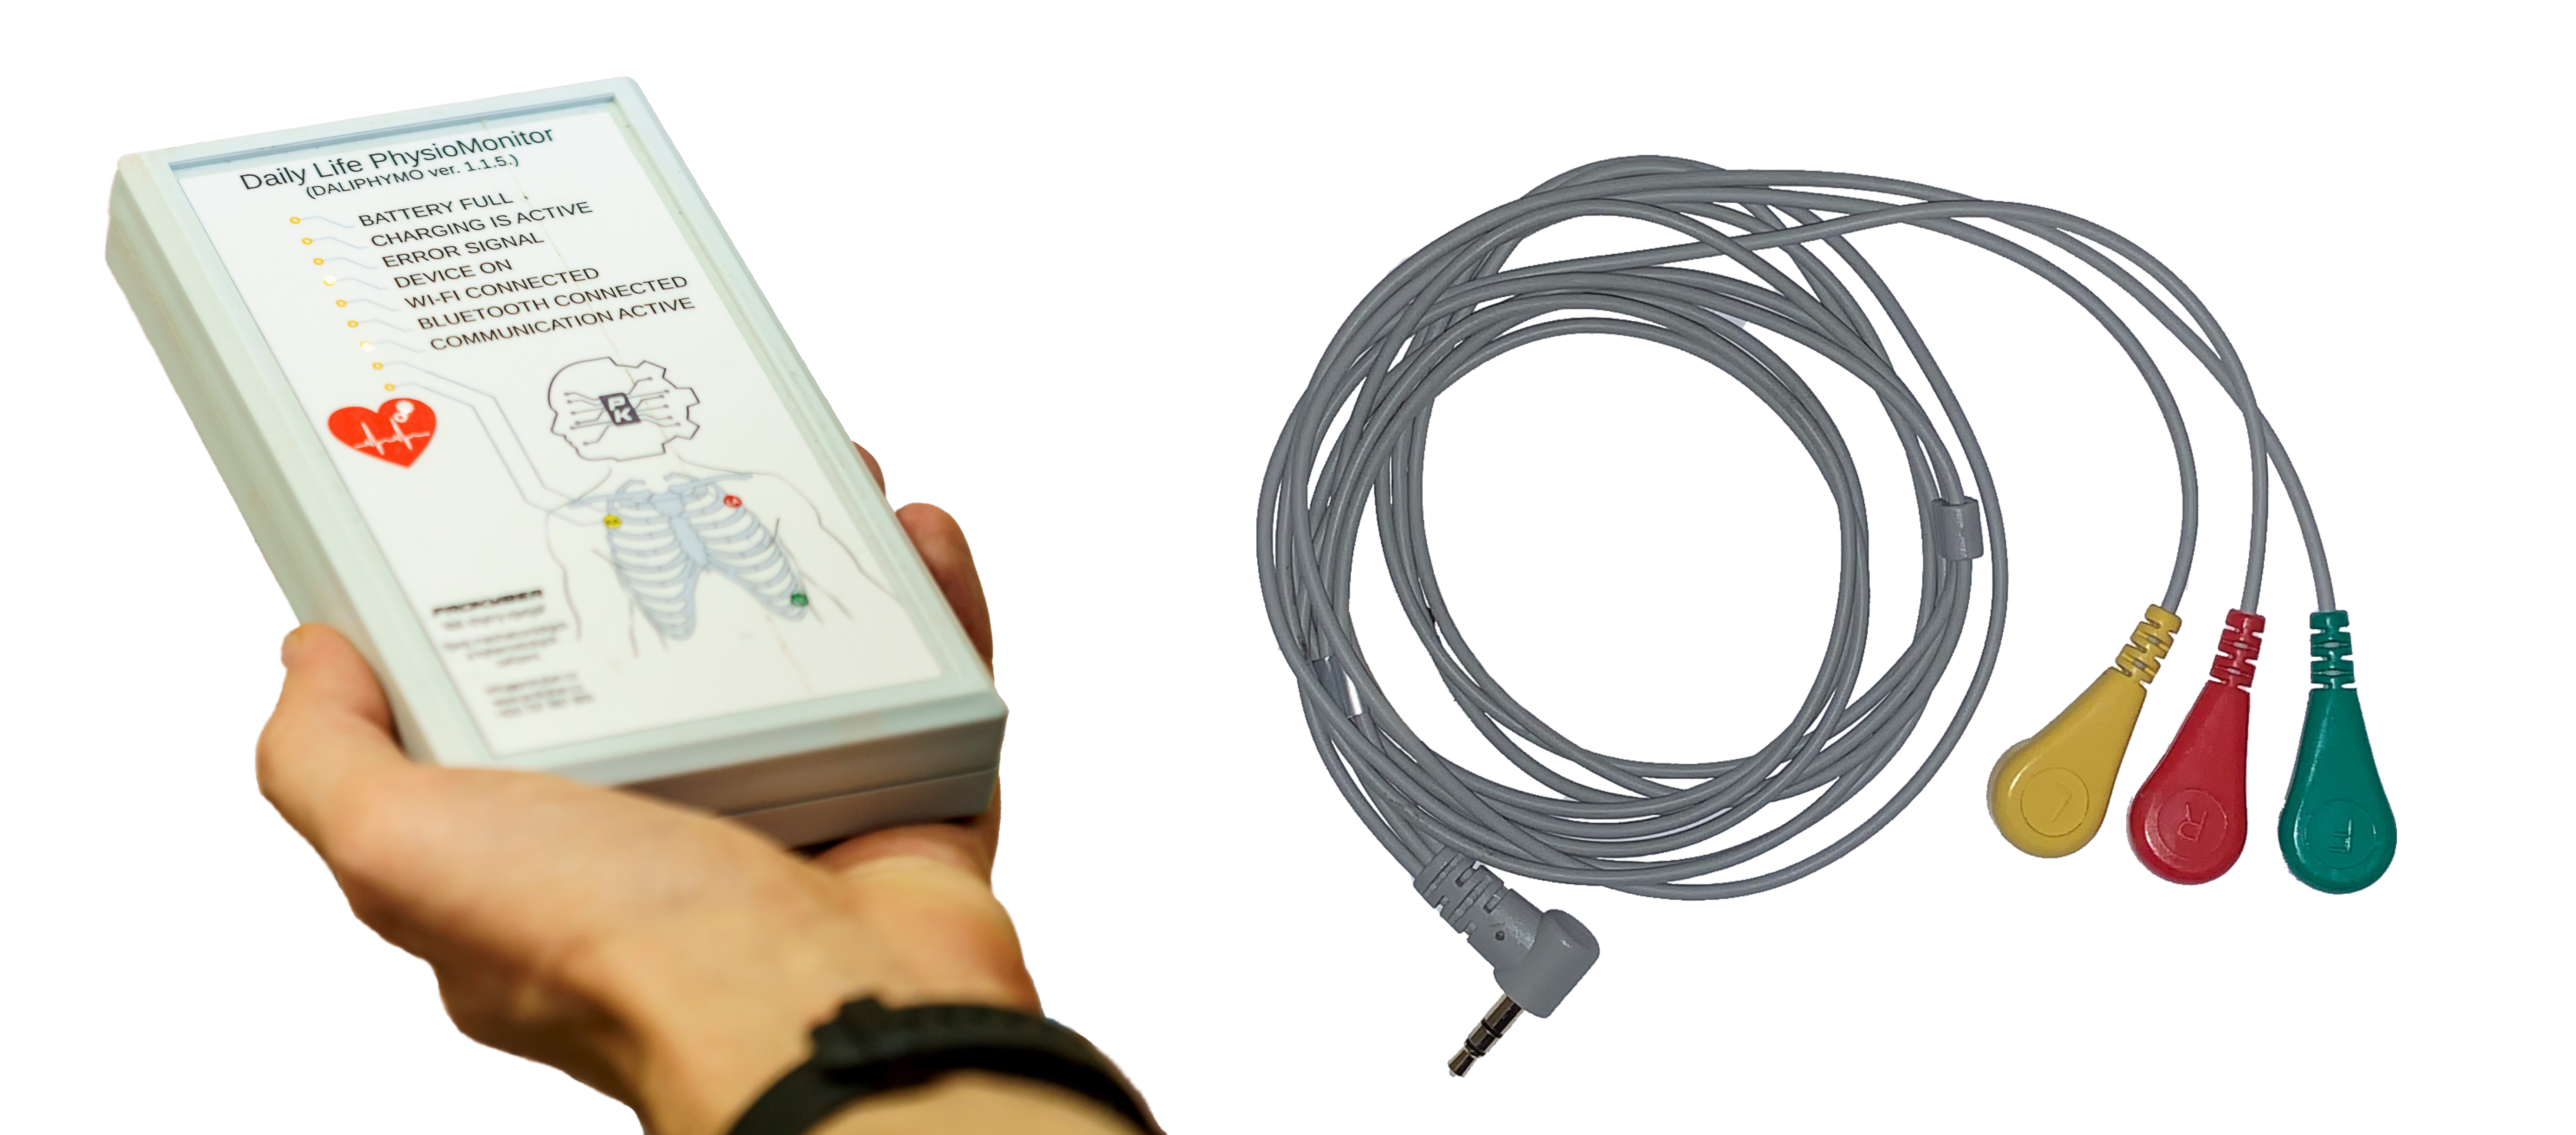
\includegraphics[width=0.9\textwidth]{../assets/device/holter1}
        \caption{Měřící zařízení s příslušenstvím}
        \label{fig:device}
    \end{center}
\end{figure}

Holterův monitor musí být při připojování k bezdrátové sítí v bezprostřední
blízkosti chytrého zařízení, kterým bude konfigurován. Postup pro připojení
měřícího zařízení k WLAN sítí je následující:
\begin{enumerate}
    \item Připojení chytrého mobilního zařízení, které bude sloužit ke
          konfiguraci Holterova monitoru, k požadované WLAN sítí, kde bude
          probíhat komunikace.
    \item Přepnutí měřícího zařízení do režimu konfigurace stiskem tlačítka
          \textbf{Config}, které se nachází na horní ploše okraje zařízení.
    \item Spuštění aplikace \textit{ESPTouch: SmartConfig}.
    \item Ověření správně vybrané WLAN sítě pomocí identifikátoru \textbf{SSID}
          v horní části úvodní obrazovky aplikace (Obr.~\ref{fig:app_screen1}).
    \item Vyplnění hesla v kolonce \textbf{Password} náležícího zvolené WLAN
          sítí. Ostatní parametry jsou ponechány ve výchozím stavu.
    \item Stisk tlačítka \textbf{Confirm} v dolní části aplikace pro zahájení
          konfigurace a připojení Holteru k vybrané sítí.
\end{enumerate}

Pokud se měřící zařízení připojilo úspěšně k vybrané WLAN sítí, objeví se
notifikace jako na Obr. \ref{fig:app_screen2} a zároveň je navázané spojení
indikované rozsvícenou LED kontrolkou na předním panelu Holteru u položky
\textbf{WI-FI CONNECTED}. Při nezdařeném pokusu připojení je nutné opakovat
kroky od bodu 2 nebo případně zkontrolovat stav baterie Holteru.

\begin{figure}[h]
    \centering
    \begin{subfigure}[b]{0.45\textwidth}
        \centering
        \textcolor{cyan}{\fboxrule=2pt\fboxsep=0pt\fbox{\includegraphics[width=0.8\linewidth]{../assets/device/app_screen1}}}
        \caption{Úvodní obrazovka aplikace}
        \label{fig:app_screen1}
    \end{subfigure}
    \hfill
    \begin{subfigure}[b]{0.45\textwidth}
        \centering
        \textcolor{cyan}{\fboxrule=2pt\fboxsep=0pt\fbox{\includegraphics[width=0.8\linewidth]{../assets/device/app_screen2}}}
        \caption{Notifikace úspěšného připojení}
        \label{fig:app_screen2}
    \end{subfigure}
    \caption{Konfigurace měřícího zařízení v aplikaci \textit{ESPTouch:
            SmartConfig}}
    \label{fig:esptouch_app}
\end{figure}

\subsubsection{Metodika měření}
\label{section:measurement_methodology}
Metodika měření spočívá v krátkodobém záznamu srdeční aktivity ve dvou odlišných
situacích. Před měřením je na subjekt připojeno měřicí zařízení, popsané v
sekci~\ref{section:measurement_device}, pomocí adhezivních EKG elektrod (viz
Obr.~\ref{fig:device_usage}). Jedná se o bipolární hrudní 3-svodové zapojení
elektrod (viz kapitola~\ref{section:electrocardiography}). Měření každého
záznamu trvá 10 minut, přičemž se jedná o dva 5 minutové spojité úseky. Subjekt
nesmí být před měřením vystaven fyzické ani psychické zátěži. Během měření v
prvním 5 minutovém úseku je subjekt po celou dobu v klidu. V druhém 5 minutovém
úseku je subjekt vystaven situaci stimulující kognitivní zátěž v podobě
Stroopova testu. Stroopův test je realizován formou videozáznamu a blíže je
popsán v následující kapitole. Postup měření je rozebrán v
sekci~\ref{section:measurement_process}.

\begin{figure}[h]
    \begin{center}
        \includegraphics[width=0.7\textwidth]{../assets/device/holter2}
        \caption{Měření srdeční aktivity}
        \label{fig:device_usage}
    \end{center}
\end{figure}

\subsubsection{Stroopův test}
\label{section:stroop_test}
Stroopův test se řadí mezi psychologické testy osobnosti a byl primárně navržený
pro testování percepční zátěže. Postupem času se možnosti jeho využití
rozšiřovaly~\cite{Svoboda1999}. Dnes je Stroopův test jeden z nejběžnějších
neuropsychologických testů používaný k hodnocení  a stimulaci kognitivní
zátěže~\cite{Scarpina2017}.

\begin{figure}[h]
    \begin{center}
        \includegraphics[width=1\textwidth]{../assets/figures/stroop}
        \caption{Příklad Stroopova testu~\cite{stroopWiki}}
        \label{fig:stroop}
    \end{center}
\end{figure}

Princip testu spočívá ve třech po sobě následujících krocích. Prvním krokem je
přečtení řady slov, která jsou napsaná černou barvou a označují několik barev
(nejčastěji červená, žlutá, zelená a modrá). Dalším krokem je pojmenování každé
jednotlivé barvy v další řadě tvořené barevnými obdélníky. Posledním krokem je
přečtení řady slov, která jsou napsaná barevně ale význam slova této barvě
neodpovídá~\cite{Svoboda1999}. Na Obr.~\ref{fig:stroop} lze vidět příklad testu.

\subsubsection{Postup měření}
\label{section:measurement_process}
Postup záznamu srdeční aktivity u jednotlivých probandů sestává z
následujících kroků:
\begin{enumerate}
    \item Konfigurace měřícího zařízení podle postupu v sekci~\ref{section:measurement_device}.
    \item Nalepení elektrod na měřeného probanda podle
          Obr.~\ref{fig:device_usage} a připojení příslušných EKG kabelů k elektrodám.
    \item Zapnutí aplikace \textit{BBPM}. Počítač na kterém běží aplikace musí
          být připojený ke stejné sítí jako měřící zařízení.
    \item Nastavení aplikace stiskem tlačítka \textbf{Settings} a vyplněním IP
          adresy a portu měřícího zařízení do kolonek \textbf{Host} a \textbf{Port} v
          kartě \textbf{General}.
    \item Ověření validity spojení stiskem tlačítka \textbf{Test connection}.
    \item Připojení aplikace k měřícímu zařízení stiskem tlačítka
          \textbf{Apply} a následně \textbf{Ok}.
    \item Zahájení záznamu srdeční aktivity stiskem tlačítka \textbf{Record} a
          vybrání cílové destinace, kde bude soubor po ukončení záznamu uložen.
    \item Ukončení záznamu po 10 minutách opětovným stiskem tlačítka \textbf{Record}.
\end{enumerate}

\subsection{Studie}
\label{section:study}
Pilotní měření EKG záznamů bylo prováděno na lidských subjektech, tudíž je nutné
mít informovaný souhlas měřených probandů a souhlasné stanovisko etické komise.

%//TODO: add reference
\subsubsection{Stanovisko etické komise}
Sběr dat proběhl v rámci výzkumu \textit{Zpátky za volant -- Diagnostický a
    rehabilitační nástroj pro osoby po poškození mozku}. Výzkum byl schválen etickou
komisí FBMI ČVUT. Stanovisko etické komise je uvedeno v Příloze A společně s
informovaným souhlasem.

\subsubsection{Kontrolní skupina probandů}
\label{section:probands}
Za účelem otestovaní navrženého řešení (viz kapitola 3) byla naměřena a
zaznamenána srdeční aktivita podle postupu~\ref{section:measurement_process} u
kontrolní skupiny 5 probandů ve věkovém rozmezí 21--23 let bez diagnostikovaných
kardiovaskulárních onemocnění.

\subsubsection{Sledované statistické veličiny}
\label{section:selected_stats_vals}
Výstupem aplikace použité k záznamu srdeční aktivity jsou soubory formátu CSV,
kde každý řádek reprezentuje naměřenou výslednou amplitudu elektrické srdeční
aktivity v daný časový okamžik. Díky znalosti vzorkovací frekvence zařízení lze
snadno ke každému záznamu vypočítat časový vektor a pracovat tak v časové
oblasti.

V závislosti na studii byly vybrány následující sledované statistické parametry
Poincarého grafu s vyžitím metody konstrukce elipsy (viz
kapitola~\ref{section:hrv_methods}):
\begin{itemize}[noitemsep]
    \item \textbf{SD1}~\textit{(Standard Deviation)} -- směrodatná odchylka R-R
          intervalů hlavní osy elipsy,
    \item \textbf{SD2}~\textit{(Standard Deviation)} -- směrodatná odchylka R-R
          intervalů vedlejší osy elipsy,
    \item \textbf{SD1/SD2}~\textit{(Standard Deviation ratio)} -- poměr směrodatných odchylek SD1 a SD2.
\end{itemize}

\subsection{Offline zpracování EKG záznamu}
\label{section:offline_processing}
Zpracování EKG záznamů se orientuje podle diagramu na Obr.
\ref{fig:diagram_offline_processing} a je realizováno v prostředí programu
\textit{MathWorks MATLAB 2021a}~\cite{MATLAB} s pomocí \textit{Signal Processing
    Toolboxu}~\cite{matlabSPT}. Jednotlivé částí zpracování jsou rozebrány v
následujících kapitolách.

\begin{figure}[H]
    \centering
    \begin{tikzpicture}[node distance=2.5cm, thick, scale=0.8, every node/.style={scale=0.8}]
        \node (start) [startstop, text width=2cm] {EKG záznam};
        \node (pro1) [process, right of=start, xshift=1.5cm] {Předzpracování};
        \node (pro2) [process, right of=pro1, xshift=1.5cm, text width=3cm] {Detekce komponentů};
        \node (pro3) [process, right of=pro2, xshift=1.5cm, text width=3cm] {Zpracování komponentů};
        \node (stop) [startstop, right of=pro3, xshift=1.5cm, text width=3cm] {Hodnocení záznamu};

        \draw [arrow] (start) -- (pro1);
        \draw [arrow] (pro1) -- (pro2);
        \draw [arrow] (pro2) -- (pro3);
        \draw [arrow] (pro3) -- (stop);
    \end{tikzpicture}
    \caption{Diagram offline zpracování EKG záznamu}
    \label{fig:diagram_offline_processing}
\end{figure}

\subsubsection{Předzpracování signálu}
\label{section:preprocessing}
Nezbytný krok pro jakoukoliv další práci s biosignálem, je jeho filtrace. Před
navržením samotného filtru byl proveden rozbor EKG záznamů pomocí FFT. EKG
signál je tak převeden z časové domény do frekvenční funkcí
\texttt{fft(X)}~\cite{matlabFFT}. Z teorie je známo v jakých frekvencích se
vyskytuje užitečný EKG signál nebo jeho komponenty a v jakých nežádoucí vlivy
(viz kapitola~\ref{section:ecg_processing_theory}). Tyto znalosti byly při
návrhu filtru a posuzování spektra EKG signálu využity. Pro zlepšení představy o
potenciálních artefaktech a užitečných frekvencích byla provedena FFT analýza i
na několika samotných PQRST segmentech. Na Obr.~\ref{fig:spectral_analysis} lze
vidět FFT analýzu EKG signálu a jednoho PQRST segmentu. Z examinace pouhé
vizuální stránky signálu plyne několik východisek pro tvorbu filtru. Jsou zde
pohybové artefakty společně s kolísáním nulové izolinie. Ve frekvenčním spektru
a v částech signálu se dále objevuje nepatrný širokopásmový šum, způsobený
myopotenciály. Ve frekvenčním spektru lze vidět tyto nežádoucí složky přibližně
mezi frekvencemi od 0 do 5--10~\si\Hz.

\begin{figure}[h]
    \begin{center}
        \includegraphics[width=1\textwidth]{../assets/figures/spectral_analysis}
        \caption{FFT analýza EKG signálu a QRS komplexu}
        \label{fig:spectral_analysis}
    \end{center}
\end{figure}

Po FFT analýze byl pro potlačení nežádoucích prvků použit pro každý EKG záznam
digitální filtr FIR typu pásmová propust s propustnými frekvencemi v rozmezí
7,5--35~\si\Hz. Filtr byl navržen metodou Kaiserova okna~\cite{Chavan2006},
které je definované~\cite{Oppenheim1999}:
\begin{equation}
    \label{eq:kaiser1}
    w[n] =
    \begin{cases}
        \frac{I_0[\beta(1-[(n-\alpha/\alpha]^2)^{1/2}]}{I_0(\beta)}, & 0 \leq n \leq M \\
        0,                                                           & \text{jinak}.
    \end{cases}
\end{equation}
kde $w$ označuje vypočítané koeficienty, $M$ je počet vzorků, $\alpha=M/2$ a
$I_0(\cdot)$ reprezentuje 0. řád modifikované Besselovy funkce prvního
druhu~\cite{BesselFcn}. Jelikož je potřeba dosáhnout specifického útlumu $A$
(viz kapitola~\ref{section:ecg_processing_theory}), definoval Kaiser parametr
$\beta$ k úpravě zvlnění propustného a závěrného pásma
následovně~\cite{Oppenheim1999}:
\begin{equation}
    \beta =
    \begin{cases}
        0.1102(A-8.7),                    & A > 50            \\
        0.5842(A-21)^0.4 + 0.07886(A-21), & 21 \leq A \leq 50 \\
        0.0,                              & A < 21.
    \end{cases}
\end{equation}

Filtr byl realizován funkcí \texttt{bandpass(x,fpass,fs)}~\cite{matlabBANDPASS}.
Druhou části předzpracování tvoří filtrace zvýrazňující QRS komplexy, konkrétně
R vlny. Použitá metoda pro zvýraznění vychází z vlastností derivace a vyšších
amplitud R vln. Filtrovaný signál je diferencován použitím pěti-bodové diference
prvního řádu dle následujícího vztahu:
\begin{equation}
    \label{eq:differentiation}
    y[n] = \frac{1}{8}(2x[n] + x[n-1] - x[n-3] - 2x[n-4])
\end{equation}
kde $n \geq 5$, $y[n]$ reprezentuje vzorek diferencovaného signálu a $x[n]$
hodnotu původního vzorku. Diferenciace zároveň potlačuje vlivy P a T vln.
Výstupem diference je bipolární signál, který je umocněn. QRS regiony jsou
následně jednotlivě sloučeny a zvýrazněny využitím zpětné
kumulace~\cite{Wang2017}:
\begin{equation}
    \label{eq:backward_cumulation}
    Bc(n) = \sum_{i=n}^{n+Ww-1} |y(i)|
\end{equation}
s pevným oknem $(Ww)$ v rozsahu nejdelšího normálního trvání jednoho QRS
komplexu (0,12~\si\s)~\cite{Wang2017}. Ke kumulaci je využívána funkce
\texttt{cumsum(A)}~\cite{matlabCUMSUM}.

\begin{figure}[h!]
    \begin{center}
        \includegraphics[width=1\textwidth]{../assets/figures/preprocessing_steps}
        \caption{Jednotlivé kroky předzpracování EKG signálu}
        \label{fig:preprocessing_steps}
    \end{center}
\end{figure}

Poslední krok předzpracování je vyhlazení vzniklých vrcholů konvolucí použitím
funkce \texttt{conv(u,v)}~\cite{matlabCONV}. Konvoluční kernel je tvořen podílem
jednotkového vektoru o délce 60 vzorků a délkou vektoru. Délka 60 vzorků je
stejně jako u zpětné kumulace doba trvání QRS komplexu, převedena z času na
počet vzorků pomocí vzorkovací frekvence (500~\si\Hz). Vizuálně lze vidět
jednotlivé kroky předzpracování signálu na Obr.~\ref{fig:preprocessing_steps}.

\subsubsection{Detekce komponentů}
\label{section:components_detection}
Detekce komponentů tvoří nezbytnou část od které se odvíjí hodnocení EKG
záznamu. Cílem detekce je spolehlivě identifikovat a lokalizovat specifické
komponenty, nejčastěji QRS komplexy, které jsou předmět analýzy EKG záznamu.
Díky detekovaným komponentům lze signál využitím detekovaných veličin
segmentovat a hodnotit. V první řadě se nejčastěji volí detekce R vln na základě
jejich vysoké amplitudy.

Za účelem detekce R vln byl implementován a modifikován algoritmus
podle~\cite{Nabian2018}, inspirovaný Pan-Tompkinsovou metodou QRS
detekce~\cite{Pan1985} (viz kapitola~\ref{section:components_detection_theory}).
Algoritmus vychází z následujících kroků:
\begin{enumerate}
    \item Iterativní hledání globálních maximálních amplitud s použitím
          plovoucího okna $W$ o délce 400~\si\ms~(0,4~\si\s):
          \begin{gather}
              R_max = max(W_i^{L,R}) \nonumber \\
              L = R = \frac{0.4~Fs}{2}, \quad L,R \in \mathbb{Z^+} \nonumber \\
              W_i^{L,R} = \{x_{i-L},...,x_i,...,x_{i+R}\}, \quad \forall i \in \{1+L,...,N-R\}
          \end{gather}
          kde $N$ je počet detekovaných R vln, $Fs$ vzorkovací frekvence, $R_i$
          potenciální R vlna, $x_i$ střed okna a $L$ spolu s $R$ posun od středu
          plovoucího okna. Nalezená maxima nacházející se uprostřed plovoucího
          okna jsou označeny jako potenciální R vlny.
    \item Eliminace všech R vln nižších než než prahová hodnota $Th_{Amp}$, která je v
          každé iteraci rovna 75 \% z průměru amplitůd posledních 8 detekovaných
          R vln. Iniciálně je prahová hodnota $Th_{Amp}$ nastavena jako:
          \begin{gather}
              n = 2~Fs, \quad n \in \mathbb{Z^+} \nonumber \\
              Th_{Amp} = \frac{1}{3} max(\{x_1,x_2,x_3,...,x_n\})
          \end{gather}
    \item Výpočet R-R intervalů ($RR_i$) diferencí detekovaných R vln ($R_i$):
          \begin{equation}
              RR_i = R_{i} - R_{i-1}, \quad \forall i \in \{2,...,N\}
          \end{equation}
          Následně je provedena iterativní kontrola vypočítaných R-R intervalů.
          Intervaly delší než prahová hodnota $Th_{RR}$ indikují chybějící R
          vlnu, která je doplněna jako maximální amplituda v rozmezí délky
          plovoucího okna následovně:
          \begin{gather}
              n = \frac{0.4~Fs}{2}, \quad n \in \mathbb{Z^+} \nonumber \\
              R_m = max(\{R_{i+n},...,R_i,...,R_{i+1-n}\}), \quad \forall i \in \{1,...,N\}
          \end{gather}
          kde $R_m$ je doplněná R vlna. Prahová hodnota $Th_{RR}$ je počátečně
          nastavena jako:
          \begin{equation}
              Th_{RR} = 1.66~RR_1
          \end{equation}
\end{enumerate}

Délka plovoucího okna se řídí fyziologickým limitem hodnoty srdečního rytmu v
případech jako jsou například supraventrikulární tachykardie (SVT) nebo flutter
síní, kde dosahuje srdeční frekvence přibližně 300 úderů za minutu (5 úderů za
sekundu)~\cite{Haberl2012,Goldberger2017}. Dva sousední QRS komplexy se tedy
nemůžou vyskytnout blíže než 200~\si\ms.

Další vlny EKG signálu (P, Q, S, T) je možné lokalizovat vztažením
fyziologických časových hodnot těchto komponentů k nalezeným R
vlnám~\cite{Nabian2018}. Na Obr.~\ref{fig:detection} lze vidět zeleně vyznačený
adaptivní práh, který se mění podle 2. kroku výše a doplněnou R vlnu, která
nebyla detekovaná v 1. kroku ale až ve 3. a následně doplněna.

\begin{figure}[h]
    \begin{center}
        \includegraphics[width=1\textwidth]{../assets/figures/detection}
        \caption{Detekce R vln}
        \label{fig:detection}
    \end{center}
\end{figure}

Aby bylo možné detekované vlny zobrazit v původním signálu jako je tomu na
Obr.~\ref{fig:detection}, byla zavedena metoda relokalizace, která upraví pozice
detekovaných R vln tak, aby souhlasily v původním EKG záznamu. Díky tomu lze
vizuálně ověřit spolehlivost algoritmu nebo evaluovat detekci v pochybných
oblastech, které jsou více zatížené nežádoucími vlivy. Postup metody se řídí
diagramem na Obr.~\ref{fig:fixpeaks}, kde $X$ reprezentuje množinu hodnot EKG
signálu.

\begin{figure}[h]
    \begin{center}
        \includegraphics[width=0.8\textwidth]{../assets/diagrams/fixpeaks}
        \caption{Relokalizace nalezených R vln}
        \label{fig:fixpeaks}
    \end{center}
\end{figure}

\subsubsection{Zpracování detekovaných komponentů}
\label{section:components_processing}
V případě analýzy variability srdečního rytmu (viz kapitola~\ref{section:hrv})
je nutné tuto veličinu vypočítat z detekovaných komponentů. Diferencí mezi
sousedícími R vlny v čase jsou vypočítány R-R intervaly neboli časová
variabilita mezi jednotlivými údery srdce. Stejně jako EKG záznam, tak i R-R
intervaly jsou zatížené artefakty a mohou představovat abnormální hodnoty.
Zdrojem artefaktů jsou nejčastěji falešně nebo nesprávně detekované či chybějící
R vlny a ektopický rytmus, který společně s invalidně detekovanými R vlny
vytváří sekvence dlouhých a krátkých srdečních period. Vizuálně lze artefakty
identifikovat jako velké náhle změny či kolísání v grafu jako je tomu na
Obr.~\ref{fig:hrv_artifacts}. Podmínkou HRV analýzy je tedy použití N-N
intervalů (normal-to-normal), které představují korigované R-R intervaly.
Korekcí je myšleno potlačení nežádoucích artefaktů.

\begin{figure}[h]
    \begin{center}
        \includegraphics[width=1\textwidth]{../assets/figures/hrv_artifacts}
        \caption{HRV zatížené artefakty}
        \label{fig:hrv_artifacts}
    \end{center}
\end{figure}

K zajištění spolehlivé HRV analýzy a minimalizaci chyb byla implementována
automatická metoda pro detekci a korekci artefaktů HRV
podle~\cite{Lipponen2019}. Metoda je založená na adaptivním prahování s využitím
dvou pohyblivých prahových hodnot. V prvním kroku je vypočtena časová diference
všech detekovaných R-R intervalů $dRRs$, která slouží k rozlišení ektopických a
nesprávně detekovaných R vln od normálního sinusového rytmu~\cite{Lipponen2019}:
\begin{gather}
    dRRs_1 = 0 \nonumber \\
    dRRs_j = RR_j - RR_{j-1}, \quad \forall j \in \{2,...,N\}
\end{gather}
kde $N$ je počet R-R intervalů. Pro detekci abnormálních intervalů je nastaven
první práh $Th1$, který se adaptuje statistickým odhadem z časově proměnného
rozdělení $dRRs$ hodnot. Práh představuje sérii hodnot, definovaných produktem
faktoru $\alpha$ a mezikvartilového rozpětí $QD$ 91 okolních $dRRs$ intervalů
následovně~\cite{Lipponen2019}:
\begin{equation}
    Th1 = \alpha~QD(|\{dRRs_{j-45},...,dRRs_{j+45}\}|), \quad \forall j \in \{1,...,N\}
\end{equation}
kde $\alpha$ je bezrozměrný škálovací faktor jehož hodnota byla globálně zvolena
5,2. Časová série $dRRs$ je následně normalizována prahovými
hodnotami~\cite{Lipponen2019}:
\begin{equation}
    dRR_j = \frac{dRRs_j}{Th1_j}, \quad \forall j \in \{1,...,N\}
\end{equation}

Veličiny $dRR$ jsou použité pro detekci ektopických, krátkých, dlouhých nebo
jednotlivě chybějících srdečních period porovnáním $|dRR|>1$. Pro zbylé případy
falešně pozitivní detekce R vln nebo jiných chyb, které nelze detekovat použitím
$dRR$, je definována série $mRRs$ jako rozdíl jednotlivých R-R intervalů a
mediánu 11 okolních hodnot~\cite{Lipponen2019}:
\begin{equation}
    mRRs_j = RR_j - median(\{RR_{j-5},...,RR_{j+5}\}), \quad \forall j \in \{1,...,N\}
\end{equation}

Vzhledem k tomu že při srdeční frekvenci 60 bpm se $mRRs$ pohybuje okolo
--0,5~\si\s~v rámci falešně pozitivní detekce srdečního cyklu a při detekci
vynechaného cyklu se blíží k 1~\si\s, tak nelze použít jednotný práh. Aby bylo
možné použít stejný práh pro všechny případy identifikace artefaktu jako v
předešlé sérii $dRRs$, jsou hodnoty $mRRs$ upravené následující
podmínkou~\cite{Lipponen2019}:
\begin{equation}
    mRRs_j =
    \begin{cases}
        2~mRRs_j, & \forall mRRs_j < 0    \\
        mRRs_j,   & \forall mRRs_j \geq 0
    \end{cases}
    , \quad \forall j \in \{1,...,N\}
\end{equation}

Při stejné srdeční frekvence (60 bpm) se hodnoty $mRRs$ po úpravě blíží k
0~\si\s~u normálního sinusového rytmu, 1~\si\s~ u vynechaných cyklů a k
--1~\si\s~ u nadbytečně detekovaných srdečních period. Stejně jako pro předchozí
sérii $dRRs$, tak i pro $mRRs$ je zaveden totožně definovaný práh
$Th2$~\cite{Lipponen2019}:
\begin{equation}
    Th2 = \alpha~QD(|\{mRRs_{j-45},...,dRRs_{j+45}\}|), \quad \forall j \in \{1,...,N\}
\end{equation}
a hodnoty $mRRs$ jsou následně normalizovány~\cite{Lipponen2019}:
\begin{equation}
    mRR_j = \frac{mRRs_j}{Th1_j}, \quad \forall j \in \{1,...,N\}
\end{equation}

Prahové hodnoty $Th1$ a $Th2$ vycházejí z předpokladu, že časová řada R-R
intervalů pochází z normálního rozdělení, který ve většině případech není
splněn, a proto dochází k chybným identifikacím artefaktů. K zamezení těchto
chyb je metoda doplněna klasifikačním rozhodovacím algoritmem, který se řídí dle
diagramu~\cite{Lipponen2019}:

\begin{figure}[h]
    \begin{center}
        \includegraphics[width=1\textwidth]{../assets/diagrams/rr_decision}
        \caption{Rozhodovací algoritmus~\cite{Lipponen2019}}
        \label{fig:rr_decision}
    \end{center}
\end{figure}

Veličiny $c_1$ a $c_2$ jsou globálně nastavené konstanty
podle~\cite{Lipponen2019}. Hodnoty $S11$ a $S12$ jsou definované v následujícím
odstavci.

Ektopické rytmy se v sérii hodnot $dRR$ projevují jako sekvence záporné, kladné
a záporné hodnoty (NPN, negative positive negative) nebo kladné, záporné a
kladné (PNP, positive negative positive). Pomocí těchto vzorů je rozlišen
ektopický rytmus od vynechaných či nadbytečných srdečních cyklů nebo náhlých
změn srdeční frekvence. Pro účely vizuálního hodnocení detekce ektopických
srdečních stahů je vytvořen dvoudimenzionální prostor $S1$
následovně~\cite{Lipponen2019}:
\begin{gather}
    S11_j = dRR_j, \quad \forall j \in \{1,...,N\} \nonumber \\
    S12_j =
    \begin{cases}
        max(\{dRR_{j-1}, dRR_{j+1}\}), & dRR_j > 0 \\
        min(\{dRR_{j-1}, dRR_{j+1}\}), & dRR_j < 0
    \end{cases}
    , \quad \forall j \in \{2,...,N\}
    \label{eq:subspace1}
\end{gather}
ve kterém se hodnoty $S11$ a $-S12$ zvětšují v rámci determinace NPN vzorem a
zmenšují u PNP případů. Na Obr.~\ref{fig:rr_process} lze vidět vizualizované
prostory $S1$ a $S2$ s vyznačenými hranicemi, vymezující detekované artefakty
podle~\eqref{eq:subspace1} a~\eqref{eq:subspace2}.

\begin{figure}[h]
    \begin{center}
        \includegraphics[width=1\textwidth]{../assets/figures/rr_process}
        \caption{Vizualizace detekovaných artefaktů}
        \label{fig:rr_process}
    \end{center}
\end{figure}

Dlouhé srdeční cykly včetně případů nedetekovaných R vln se projevují v $dRR$
sérii sekvencí PN, pomalé cykly NP a nadbytečné periody jako NNP nebo NPP. K
zobrazení těchto artefaktů a jejich detekčních hranic slouží 2D prostor $S2$
definovaný~\cite{Lipponen2019}:
\begin{gather}
    S21_j = dRR_j, \quad \forall j \in \{1,...,N\} \nonumber \\
    S22_j =
    \begin{cases}
        min(\{dRR_{j-1}, dRR_{j+1}\}), & dRR_j \geq 0 \\
        max(\{dRR_{j-1}, dRR_{j+1}\}), & dRR_j < 0
    \end{cases}
    , \quad \forall j \in \{2,...,N\}
    \label{eq:subspace2}
\end{gather}

Posledním krokem je korekce detekovaných artefaktů, která se řídí jejich typem a
následný přepočet nové série korigovaných R-R intervalů. Úprava je realizována
pro každý typ artefaktu následujícím způsobem~\cite{Lipponen2019}:
\begin{itemize}
    \item \textbf{Falešně pozitivní srdeční periody} -- odstranění
          nadbytečných, nesprávně detekovaných R vln, které jsou začátkem falešné
          periody.
    \item \textbf{Vynechané srdeční periody} -- přidání nových R vln, které
          rovnoměrně rozdělí korespondující R-R interval.
    \item \textbf{Dlouhé a krátké srdeční periody} -- interpolace a přidání
          nových R-R intervalů.
    \item \textbf{Ektopický rytmus} -- nahrazení ektopických period interpolovanými R-R intervaly.
\end{itemize}

\subsubsection{Analýza zpracovaného záznamu}
\label{section:analysis}
Pro analýzu EKG záznamů, konkrétně hodnocení HRV, byla zvolena nelineární
geometrická metoda Poincarého grafu s konstrukcí elipsy (viz
kapitola~\ref{section:hrv_methods}). Jedná se o bodový graf, kde každý bod tvoří
R-R interval vynesený proti následujícímu R-R intervalu. Prvním krokem k
sestrojení grafu je vytvoření časových vektorů následovně~\cite{Mazhar2007}:
\begin{gather}
    \overrightarrow{RR_i} = \{RR_1, RR_2,...,RR_{N}\} \\
    \overrightarrow{RR_{i+1}} = \{RR_2, RR_3,...,RR_{N-1}\}
\end{gather}
kde $N$ je celkový počet R-R intervalů. Dalším krokem je výpočet kvantitativních
parametrů Poincarého grafu $SD1$ a $SD2$, které zároveň slouží ke konstrukci
elipsy. Směrodatné odchylky $SD1$ a $SD2$ jsou vypočteny jako~\cite{Mazhar2007}:
\begin{equation}
    SD1 = \sqrt{var(x1)}
    \quad \textrm{a} \quad
    SD2 = \sqrt{var(x2)}
\end{equation}
kde $x_1$ a $x_2$ neboli hlavní a vedlejší osa elipsy jsou
rovny~\cite{Mazhar2007}:
\begin{equation}
    x_1 = \frac{\overrightarrow{RR_i}-\overrightarrow{RR_{i+1}}}{\sqrt(2)}
    \quad \textrm{a} \quad
    x_2 = \frac{\overrightarrow{RR_i}-\overrightarrow{RR_{i+1}}}{\sqrt(2)}
\end{equation}

\noindent Elipsa je konstruována využitím jejího vyjádření parametrickými
rovnicemi:
\begin{gather}
    \label{eq:ellipse_parametric}
    x = a \cos \theta \nonumber \\
    y = b \sin \theta
\end{gather}
kde $\theta \in \langle 0, 2\pi \rangle$, $a$ je šířka elipsy a $b$ je její
výška. Za výšku elipsy je dosazena hodnota $SD1$ a za šířku $SD2$. Hlavní osa
elipsy leží v případě Poincarého grafu na přímce dané předpisem $y=x$ a elipsa
je tak natočena o 45\degree~($\frac{\pi}{4}$). Vypočítané body z parametrického
vyjádření elipsy~(\ref{eq:ellipse_parametric}) je tedy nutné
rotovat následovně:
\begin{equation}
    \begin{bmatrix}
        X \\
        Y
    \end{bmatrix}
    =
    \overline{RR} +
    \begin{bmatrix}
        \cos \frac{\pi}{4} & -\sin \frac{\pi}{4} \\
        \sin \frac{\pi}{4} & \cos \frac{\pi}{4}
    \end{bmatrix}
    \cdot
    \begin{bmatrix}
        x \\
        y
    \end{bmatrix}
\end{equation}
kde $X$ a $Y$ jsou výsledné body po rotaci o 45\degree. $\overline{RR}$ je
vypočítaný průměr z R-R intervalů a je středem elipsy, do kterého je třeba
elipsu posunout přičtením této hodnoty k oběma souřadnicím. Proměnné $x$ a $y$
jsou předešle vypočítané souřadnice podle~\ref{eq:ellipse_parametric}.

\bigskip

\begin{figure}[h]
    \begin{center}
        \includegraphics[width=0.65\textwidth]{../assets/figures/my_poincare}
        \caption{Realizace Poincarého grafu s elipsou}
        \label{fig:my_poincare}
    \end{center}
\end{figure}

\subsection{Online zpracování EKG záznamu}
\label{section:online_processing}
Pro zpracování EKG signálu v reálném čase bylo naprogramované multiplatformní
řešení s grafickým učitelským rozhraním (GUI) pojmenované \textit{BBPM -- Better
    bpm}. Zpracování signálu se se řídí stejným diagramem jako v
kapitole~\ref{section:offline_processing} na
Obr.~\ref{fig:diagram_offline_processing}. Motivací pro vznik aplikace je
spolupráce s Mgr. et Mgr. Ivetou Fajnerovou, Ph.D. z Národního ústavu duševního
zdraví (NÚDZ). Aplikace je využívána pro hodnocení duševního stavu osob ve
virtuální realitě. Detailněji je program popsán v následujících kapitolách.

\subsubsection{Aplikace pro hodnocení a sběr dat}
Program byl vytvořen pomocí skriptovacího programovacího jazyka
\textit{Python}~\cite{python} s využitím frameworku \textit{PySide2} (viz
sekce~\ref{section:pyside}). Hlavním účelem programu je online zpracovaní a
vizualizace dat z měřícího zařízení, aby bylo možné sledovat a hodnotit
elektrickou srdeční aktivitu měřené osoby v reálném čase. Aplikací lze data i
zaznamenávat a vzápětí uložit ve formátu CSV. K zajištěni minimální latence mezi
vizualizací zpracovaných dat a přijatými aktuálními daty, probíhá zpracování
signálu, jeho analýza a záznam paralelně (tzv. multithreading).

\subsubsection{Struktura aplikace}
Aplikaci lze rozdělit na dvě základní rozhraní, frontend a backend. Frontendová
část poskytuje interaktivní GUI společně s vizualizací zpracovaných dat (viz
kapitoly~\ref{section:gui}~a~\ref{section:visual}). V backendu probíhá v
jednotlivých vláknech (threadech) akvizice a záznam dat včetně výpočetních
procesů spojených se zpracováním EKG signálu (viz
sekce~\ref{section:online_data_process}). Strukturu aplikace lze vidět na
Obr.~\ref{fig:app_structure}.

\begin{figure}[h]
    \begin{center}
        \includegraphics[width=0.9\textwidth]{../assets/diagrams/app_structure}
        \caption{Struktura aplikace \textit{BBPM}}
        \label{fig:app_structure}
    \end{center}
\end{figure}

\subsubsection{PySide framework}
\label{section:pyside}
\textit{PySide} představuje vazbu (binding) skriptovacího jazyka \textit{Python}
na sadu GUI nástrojů populární knihovny \textit{Qt} \cite{Qt}. Díky tomu je
možné využívat aplikační rozhraní (API) knihovny \textit{Qt} v prostředí
\textit{Python}. \textit{Qt} není pouze knihovna ale celý nativní
multiplatformní framework pro vytváření softwaru s GUI, napsaný v programovacím
jazyce \textit{C++}. V aplikaci \textit{BBPM} byla použita knihovna
\textit{PySide2}, která představuje port pro \textit{Qt5}.

\subsubsection{Uživatelské rozhraní}
\label{section:gui}
Grafické uživatelské rozhraní zajišťuje jednoduchou komunikaci mezi aplikací a
uživatelem pomocí interaktivních komponentů. Pro návrh a tvorbu GUI byl použit
nástroj \textit{Qt Designer}~\cite{QtDesigner}, který je součástí knihovny
\textit{PySide2} a lze vidět na Obr.~\ref{fig:qt_designer}. Nástroj funguje na
principu \textit{WYSIWYG} editorů a umožňuje tak rychlou a intuitivní tvorbu
uživatelského rozhraní. V prostředí nástroje je vidět živý náhled aplikace v
podobě uživatelského okna~(\ref{fig:qt_designer}--\textbf{3}), které je hlavním
komponentem. Do hlavního okna lze z panelu č.~\textbf{1} přesouvat interaktivní
uživatelské prvky. Jednotlivé parametry prvků společně s hlavním oknem (např.
výška a šířka) lze upravovat v panelu č.~\textbf{2}. Vytvořené GUI je možné
následně exportovat v podobě \textit{Python} kódu.

\begin{figure}[h]
    \begin{center}
        \includegraphics[width=1\textwidth]{../assets/bbpm/qt_designer}
        \caption{Prostředí \textit{Qt Designeru}}
        \label{fig:qt_designer}
    \end{center}
\end{figure}

Pro potřeby aplikace byly vytvořeny dvě okna -- hlavní okno a okno nastavení.
Hlavní okno (viz Obr.~\ref{fig:app_main_window}) se skládá z postranního
vysouvacího menu~(\ref{fig:app_main_window}-\textbf{1}), které se nachází na
levé straně okna a panelu~(\ref{fig:app_main_window}-\textbf{2}), ve kterém se
zobrazuje karta podle zvolené položky v menu. Vysouvací menu obsahuje čtyři
tlačítka, přičemž první tlačítko, které se nachází v levém horním rohu hlavního
okna, iniciuje vysunutí a zasunutí menu. Jednotlivé funkce ostatních tlačítek
jsou:
\begin{itemize}[noitemsep]
    \item \textbf{Dashboard} -- zobrazení hlavní karty vizualizující výstup,
    \item \textbf{Record} -- zapnutí nahrávání EKG záznamu,
    \item \textbf{Settings} -- vyvolání dialogového okna s nastavením.
\end{itemize}
Postranní menu je modulární, což umožňuje snadné přidání nových položek a k nim
přidružených karet v pravém panelu. Modularita některých funkcí aplikace tak
zajišťuje snadnou rozšířitelnost v budoucnu.

\begin{figure}[h]
    \begin{center}
        \includegraphics[width=1\textwidth]{../assets/bbpm/main_window}
        \caption{Struktura hlavního okna aplikace}
        \label{fig:app_main_window}
    \end{center}
\end{figure}

Karta \textbf{Dashboard} se skládá ze dvou segmentů. Dolní segment karty je
tvořen grafem pro zobrazení EKG křivky~(\ref{fig:app_main_window}-\textbf{4}),
který je detailněji popsán v sekci~\ref{section:visual}. Horní
segment~(\ref{fig:app_main_window}-\textbf{3}) obsahuje čtyři informační
subpanely. První tři zobrazují aktuální srdeční frekvenci, průměrnou srdeční
frekvenci a průměrnou délku R-R intervalů za posledních 6 sekund. První subpanel
zobrazující srdeční frekvenci, zároveň barevně indikuje, zda je její hodnota ve
fyziologickém rozmezí (zelená) nebo je zvýšená, snížená (oranžová) či abnormální
(červená). Rozmezí hodnot bylo zvoleno na základě stanoviska Americké
kardiologické asociace (AHA).

\begin{table}[h]
    \captionsetup{font=small,skip=0.5pt}
    \label{tab:aha_table}
    \catcode`\-=12
    \begin{center}
        \caption{Stanovené hodnoty srdeční frekvence podle AHA}
        \vspace{1ex}
        \setlength{\tabcolsep}{20pt}
        \renewcommand{\arraystretch}{1.3}
        \begin{tabular}{lcc}
            \noalign{\hrule height 2pt}
            \textbf{Srdeční rytmus} &  & \textbf{hodnota (bpm)} \\ \hline
            Bradykardie             &  & < 60                   \\
            Normální                &  & 60--100                \\
            Tachykardie             &  & > 100                  \\ \noalign{\hrule height 2pt}
        \end{tabular}
    \end{center}
\end{table}

Poslední informační subpanel (Events) má uplatnění během měření a hodnocení osob
ve VR v rámci výzkumu \textit{Virtuální město – herní systém pro kognitivní
    trénink ve virtuálním prostředí}, zmíněného v úvodu
kapitoly~\ref{section:online_processing}. V této práci nemá využití, a proto
není dále blíže popsán.

Okno nastavení obsahuje čtyři záložky (viz Obr. \ref{fig:settings_cards}):
\begin{itemize}
    \item \textbf{General} (Obr.~\ref{fig:settings_general}) -- slouží pro
          nastavení připojovacích údajů k měřícímu zařízení. Tlačítkem \textbf{Test
              connection} lze zkontrolovat připojení.
    \item \textbf{Graph} (Obr.~\ref{fig:settings_graph}) -- slouží k nastavení
          grafu, konkrétně jeho vykreslovacích vlastností. Lze zde nastavit barva a
          tloušťka křivky nebo schovat osy a grid.
    \item \textbf{Recording} (Obr.~\ref{fig:settings_recording}) -- slouží k
          nastavení ID a jména měřené osoby, které se po nahrávání uloží
          společně s naměřenými daty.
    \item \textbf{Info} -- obsahuje informace o verzi aplikace a copyright.
\end{itemize}

\begin{figure}[h]
    \centering
    \begin{subfigure}[b]{0.3\textwidth}
        \centering
        \textcolor{cyan}{\fboxrule=0.5pt\fboxsep=0pt\fbox{\includegraphics[width=1.1\linewidth]{../assets/bbpm/settings_general}}}
        \caption{záložka General}
        \label{fig:settings_general}
    \end{subfigure}
    \hfill
    \begin{subfigure}[b]{0.3\textwidth}
        \centering
        \textcolor{cyan}{\fboxrule=0.5pt\fboxsep=0pt\fbox{\includegraphics[width=1.1\linewidth]{../assets/bbpm/settings_graph}}}
        \caption{záložka Graph}
        \label{fig:settings_graph}
    \end{subfigure}
    \hfill
    \begin{subfigure}[b]{0.3\textwidth}
        \centering
        \textcolor{cyan}{\fboxrule=0.5pt\fboxsep=0pt\fbox{\includegraphics[width=1.1\linewidth]{../assets/bbpm/settings_recording}}}
        \caption{záložka Recording}
        \label{fig:settings_recording}
    \end{subfigure}
    \caption{Jednotlivé záložky v okně Nastavení}
    \label{fig:settings_cards}
\end{figure}

\subsubsection{Zpracování dat}
\label{section:online_data_process}
Pro zpracování dat jsou využívané integrované funkce prostředí \textit{Python} a
knihovny \textit{SciPy}~\cite{SciPy2020}. Před zpracováním EKG signálu jsou
přijatá data nejdříve upraveny. Aplikace přijímá z měřícího zařízení v každý
jeden okamžik blok synchronizovaných dat v podobě dvou vektorů o velikosti 2048
hodnot. Jeden vektor obsahuje EKG data a druhý časové. Jednotlivě přijaté bloky
na sebe nenavazují ale překrývají se (viz Obr.~\ref{fig:bisection}).
\begin{figure}[h]
    \begin{center}
        \includegraphics[width=0.9\textwidth]{../assets/figures/bisection}
        \caption{Bisekce překrývajících se dat}
        \label{fig:bisection}
    \end{center}
\end{figure}
Kontinuita dat je zajištěna použitím algoritmu bisekce, realizovaného funkcí
\texttt{bisect(a,x)}~\cite{bisectRight}, který najde index prvního navazujícího
prvku v závislosti na poslední hodnotě časového vektoru minulého bloku dat.
Překrývající data před tímto indexem jsou odstraněna a podle takto upraveného
časového vektoru je následně upraven i vektor s EKG daty.

Upravené bloky EKG dat jsou předzpracovány filtrem
Savitzky–Golay~(SGF)~\cite{Schafer2011} použitím funkce
\texttt{savgol{\_}filter(x,win{\_}length,order)}~\cite{scipySavgol}. Filtr
Savitzky–Golay je digitální filtr s konečnou impulzní odezvou (FIR), který se
nejčastěji používá k vyhlazení signálu a potlačení vysokofrekvenčního obsahu.
Princip filtru SGF vychází z proložení hodnot v plovoucím okně polynomem
určitého řádu využitím metody nejmenších čtverců. Výsledná hodnota signálu v
daném bodě je vypočtena jako~\cite{wikiSGF}:
\begin{equation}
    y_j = \sum_{i=\frac{1-M}{2}}^{\frac{M-1}{2}} = c_j y_{j+i}, \quad \frac{M-1}{2} \leq j \leq N - \frac{M-1}{2}
\end{equation}
kde $c_j$ jsou vypočítané koeficienty polynomiální regrese, $M$ je délka
plovoucího okna a $N$ délka signálu. V aplikaci byla zvolena délka okna 151
vzorků a polynom 3. řádu. Příklad SGF filtrace se zvolenými parametry lze vidět
na Obr.~\ref{fig:sgf_filter}.

\begin{figure}[h]
    \begin{center}
        \includegraphics[width=1\textwidth]{../assets/figures/sgf_filter}
        \caption{Savitzky–Golay filtrace}
        \label{fig:sgf_filter}
    \end{center}
\end{figure}

Po filtraci jsou data přidána do cyklické fronty~\cite{circlebuffer}, kde
probíhá nepřetržitá detekce komponentů, konkrétně R vln. K detekci je používána
funkce \texttt{find{\_}peaks(x,h,d)}~\cite{scipyFindpeaks}. Funkcí probíhá
hledání lokálních maxim signálu v závislosti na zadané prahové amplitudě a
minimální vzdáleností mezi sousedními R vlny. Prahová hodnota amplitudy byla
zvolena 0,2~\si\mV~a minimální vzdálenost 0,4~\si\s~(200 vzorků).

Zpracování komponentů (R vln) se odvíjí od zobrazených parametrů na hlavním
panelu aplikace (viz Obr. \ref{fig:app_main_window}). Z detekovaných vln se
počítá aktuální srdeční frekvence z diference posledních dvou detekovaných R vln
následovně:
\begin{equation}
    \label{eq:calc_hr}
    HR = \frac{60}{RR}
\end{equation}
kde $HR$ je hodnota srdeční frekvence a $RR$ aktuálně vypočtená srdeční
perioda. Na panelu je z vypočítané hodnoty zobrazena celá část čísla. Dalším
parametrem je průměrná hodnota srdeční frekvence, která se počítá podle
vztahu~\ref{eq:calc_hr} výše. Namísto $RR$ je ale dosazena průměrná hodnota
všech R-R intervalů za posledních 6 sekund, která je posledním počítaným
parametrem podle:
\begin{equation}
    \overline{RR} = \frac{1}{N} \sum_{i=1}^N RR_i
\end{equation}
kde $\overline{RR}$ je vypočítaný průměr R-R intervalů a $N$ je počet R-R
intervalů. Hodnoty se následně zobrazují na panelu jako je tomu na
Obr.~\ref{fig:app_info_subpanels}.

\subsubsection{Vizualizace EKG}
\label{section:visual}
Pro vykreslování dat je použita knihovna \textit{PyQtGraph} \cite{PyQtGraph},
která je plně kompatibilní s frameworkem \textit{PySide2} (viz
sekce~\ref{section:pyside}). Hlavním komponentem této knihovny je graf, kterému
lze funkcí \texttt{setData(x,y)}~\cite{curveItem} předat hodnoty pro osu X a Y.
Po předání jsou hodnoty vykresleny a graf je aktualizován. Předávání hodnot je
zacykleno, a tak dochází
\begin{figure}[H]
    \begin{center}
        \includegraphics[width=0.75\textwidth]{../assets/bbpm/r_detection}
        \caption{Vizualizace EKG křivky s detekcí R vln v aplikaci}
        \label{fig:app_ecg_visual}
    \end{center}
\end{figure}
\noindent k neustálému vykreslování nových EKG dat. Zároveň jsou využity hodnoty
detekovaných R vln pro vykreslování markerů v podobě modrých šipek, které tyto
vlny označují. Vizualizace dat na hlavním panelu je vidět na
Obr.~\ref{fig:app_ecg_visual}.

\subsection{Statistické metody}
\label{section:statistical_methods}
Pro zpracování výsledků byly v práci použity statistické testy, realizovány
funkcemi v prostředí programu \textit{MathWorks MATLAB 2021a}~\cite{MATLAB},
které prověřují platnost nulové hypotézy $H_0$. Nulová hypotéza představuje ve
většině případů tvrzení, že rozdíl mezi testovanými daty není statisticky
významný. Proti $H_0$ se zavadí alternativní hypotéza $H_A$, která nulovou
hypotézu vyvrací. K určení platnosti mezi testovanou nebo alternativní hypotézou
slouží statistické testování, které probíhá následovně:
\begin{itemize}
    \item Definice nulové hypotézy $H_0$ s předpokladem, že platí.
    \item Stanovení náhodného pokusu, kterým bude ověřena hypotéza a náhodné
          veličiny, která bude výsledkem pokusu.
    \item Zvolení hladiny významnosti \textalpha, která vyjadřuje
          pravděpodobnost neoprávněného zamítnutí nulové hypotézy $H_0$, i když platí.
          V bakalářské práci je zvolena hladina významnosti \textalpha~=~0,05 (5~\%).
    \item Zamítnutí nulové hypotézy $H_0$ v případě, že hodnota náhodné veličiny
          spadá do kritického oboru, jelikož nastal jev, který by byl velmi
          nepravděpodobný za platnosti hypotézy $H_0$.
    \item Vyhodnocení statistického testu na základě rozhodnutí o platnosti
          nulové hypotézy $H_0$: přijetí hypotézy $H_0$ (zamítnutí alternativní
          hypotézy $H_A$) nebo zamítnutí hypotézy $H_0$ (přijetí alternativní
          hypotézy $H_A$).
\end{itemize}

Pro testování normality náhodné veličiny byl zvolen Shapirův-Wilkův
test~\cite{wikiSHAPIROWILK} na základě porovnání síly testů pro malé vzorky
podle~\cite{Razali2011}. Nulová hypotéza testu $H_0$ tvrdí, že testovaný vzorek
dat pochází z populace s normálním rozdělením. Test byl proveden použitím funkce
\texttt{swtest(x)}~\cite{matlabSWTEST}.

\subsubsection{Parametrické testy}
\label{section:parametric_tests}
Parametrické varianty testů mohou být uplatněny pouze v případě splnění podmínky
normality dat. V práci byl použit párový t-test~\cite{Henry2005}, který testuje
rozdíl středních hodnot mezi dvojicí veličin dvourozměrného náhodného výběru.
Test byl realizován použitím funkce \texttt{ttest(x)}~\cite{matlabTTEST}.
\clearpage

\section{Výsledky}
Kapitola výsledky je rozdělena na čtyři části. První dvě kapitoly prezentují
realizované softwarové řešení pro online a offline hodnocení srdeční aktivity.
Následně sekce~\ref{sections:results_probands} uvádí výsledky analýzy
zpracovaných záznamů a statistického testování normality sledovaných veličin
(viz kapitola~\ref{section:selected_stats_vals}).
Sekce~\ref{sections:results_analysis} popisuje výsledky statistického ověření
metody Poincarého grafu v rámci hodnocení HRV u zpracovaných EKG záznamů.

\subsection{Softwarové řešení pro offline hodnocení EKG}
\label{sections:results_online}
Výstup jednotlivých fází zpracování EKG záznamů (viz kapitola
\ref{section:offline_processing}) byl sjednocen do jednoho hlavního okna pomocí
integrovaného \textit{App Designeru} \cite{matlabAPPDESIGNER} v programovém
prostředí MATLAB. Výsledkem je spustitelná interaktivní aplikace. Po
spuštění aplikace lze v menu pomocí tlačítka \textbf{Load signal} nahrát EKG
signál ve formátu CSV nebo MAT. Po výběru EKG signálu je uživatel tázán aby
zadal vzorkovací frekvenci signálu. EKG signál je následně adaptivně zpracován.
\begin{figure}[h]
	\begin{center}
		\includegraphics[width=1\textwidth]{matlab_EDA/tab4}
		\caption{Hlavní okno aplikace -- karta HRV analysis}
		\label{fig:results_matlab_tab4}
	\end{center}
\end{figure}
Na Obr.~\ref{fig:results_matlab_tab4} lze vidět otevřenou kartu \textbf{HRV
analysis}, která vizualizuje výstup HRV analýzy vycházející ze všech předešlých
fází zpracování. Všechny karty aplikace jsou uvedené v Příloze B. Jednotlivé
karty jsou mezi sebou propojené. Pokud například uživatel v jedné kartě posune
signál na určitý čas, tak se tato změna aplikuje na signály ostatních karet.

\subsection{Softwarové řešení pro online hodnocení EKG}
\label{sections:result_offline}
Pro účely online analýzy EKG a sběr dat byla naprogramovaná aplikace jménem
\textit{BBPM} v prostředí Python. Prostředí \textit{Python} bylo
zvoleno na základě jeho open-source licence, která jej umožňuje zdarma používat
a volně nebo i komerčně distribuovat vyvinutá řešení. Aplikaci lze vidět na
Obr.~\ref{fig:results_bbpm}. Realizované řešení bylo použito pro pilotní měření
a záznam surových EKG signálů u kontrolní skupiny probandů (viz
kapitola~\ref{section:probands}). Aplikace je detailněji popsaná v
kapitole~\ref{section:online_processing}.

\begin{figure}[H]
	\begin{center}
		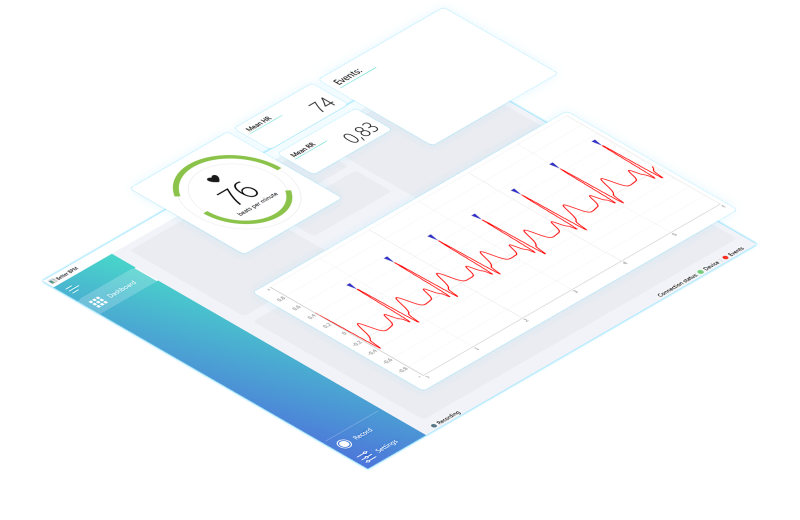
\includegraphics[width=1\textwidth]{bbpm/bbpm_app}
		\caption{Aplikace \textit{BBPM}}
		\label{fig:results_bbpm}
	\end{center}
\end{figure}

\clearpage

\subsection{Kontrolní skupina}
\label{sections:results_probands}
V rámci kontrolní skupiny (viz sekce~\ref{section:probands}) bylo dle postupu v
kapitole~\ref{section:measurement_methodology} naměřeno 5 EKG záznamů aplikací
\textit{BBPM} (\ref{section:online_processing}). Záznamy byly následně
zpracované realizovaným SW řešením popsaným v
sekci~\ref{section:offline_processing}. V následujících podkapitolách jsou
prezentovány výsledky jednotlivých fází zpracování realizovaného offline řešení
pro hodnocení EKG.

\subsubsection{Detekované R vlny}
Následující tabulka \ref{tab:detected_artifacts} uvádí výstup fáze zpracování
detekovaných komponentů společně s vypočítanými parametry: průměrná hodnota
korigovaných (normálních, N-N) R-R intervalů (mNN), průměrná hodnota srdeční
frekvence (mHR), směrodatná odchylka R-R intervalů (SDNN) a směrodatná odchylka
srdeční frekvence (SDHR). Hodnoty parametrů vychází z R vln, který byly
korigovány algoritmem popsaným v sekci~\ref{section:measurement_process}. Z
korigovaných veličin vychází následná HRV analýza. Detekované artefakty uvádí
Tab.~\ref{tab:detected_artifacts}.

\begin{table}[h]
	\captionsetup{skip=0.5pt}
	\catcode`\-=12
	\begin{center}
		\caption{\label{tab:corrected_components} Korigované R vlny s vypočítanými parametry časové série R-R intervalů z klidové částí měření (N) a při Stroopově testu (S)}
		\vspace{1ex}
		\setlength{\tabcolsep}{13pt}
		\renewcommand{\arraystretch}{1.3}
		\begin{tabular}{llccccc}
			\noalign{\hrule height 2pt}
			                    &   &                      & \multicolumn{4}{c}{\textbf{Vypočítané parametry (ms)}}                                                 \\	\cline{4-7}
			                    &   &                      & \textbf{mNN}                                           & \textbf{mHR}  & \textbf{SDNN} & \textbf{SDHR} \\
			                    &   & \textbf{Počet R vln} & \small{(ms)}                                           & \small{(bpm)} & \small{(ms)}  & \small{(bpm)} \\	\noalign{\hrule height 2pt}
			\textbf{1. proband} & N & 369                  & 957                                                    & 64            & 139           & 10            \\
			                    & S & 428                  & 1043                                                   & 58            & 114           & 7             \\	\noalign{\hrule}
			\textbf{2. proband} & N & 374                  & 1055                                                   & 57            & 101           & 6             \\
			                    & S & 270                  & 982                                                    & 62            & 81            & 5             \\	\noalign{\hrule}
			\textbf{3. proband} & N & 535                  & 635                                                    & 95            & 49            & 7             \\
			                    & S & 542                  & 586                                                    & 103           & 52            & 9             \\	\noalign{\hrule}
			\textbf{4. proband} & N & 539                  & 649                                                    & 93            & 56            & 8             \\
			                    & S & 607                  & 536                                                    & 113           & 47            & 10            \\	\noalign{\hrule}
			\textbf{5. proband} & N & 447                  & 920                                                    & 67            & 142           & 10            \\
			                    & S & 321                  & 897                                                    & 68            & 91            & 7             \\ 	\noalign{\hrule height 2pt}
		\end{tabular}
	\end{center}
\end{table}

\subsubsection{Detekované artefakty R-R intervalů}
Včetně korigovaných R vln jsou výstupními parametry fáze zpracování detekovaných
komponentů také detekované artefakty. Počty detekovaných
artefaktů za celý 10 minutový EKG záznam jsou pro každého probanda vyneseny v
Tab.~\ref{tab:detected_artifacts}. Detekce artefaktů, společně se způsoby
korekce jejich jednotlivých typů, je popsaná v
sekci~\ref{section:components_processing}.

\begin{table}[h]
	\captionsetup{skip=0.5pt}
	\catcode`\-=12
	\begin{center}
		\caption{\label{tab:detected_artifacts} Detekované artefakty v časové sérii R-R intervalů}
		\vspace{1ex}
		\setlength{\tabcolsep}{11pt}
		\renewcommand{\arraystretch}{1.3}
		\begin{tabular}{llcccc}
			\noalign{\hrule height 2pt}
			                    &  & \multicolumn{4}{c}{\textbf{Srdeční periody (počet artefaktů)}}                                                                     \\	\cline{3-6}
			                    &  & \textbf{Ektopické}                                             & \textbf{Dlouhé/krátké} & \textbf{Nadbytečné} & \textbf{Vynechané} \\	\hline
			\textbf{1. proband} &  & 2                                                              & 6                      & 1                   & 5                  \\
			\textbf{2. proband} &  & 3                                                              & 0                      & 0                   & 3                  \\
			\textbf{3. proband} &  & 7                                                              & 0                      & 0                   & 12                 \\
			\textbf{4. proband} &  & 0                                                              & 0                      & 0                   & 0                  \\
			\textbf{5. proband} &  & 0                                                              & 3                      & 0                   & 3                  \\	\noalign{\hrule height 2pt}
		\end{tabular}
	\end{center}
\end{table}

\subsection{Analýza EKG záznamu pomocí Poicarého grafu}
\label{sections:results_analysis}
Pro kvantitativní hodnocení srdeční aktivity pomocí Poincarého grafu počítá
realizovaná MATLAB aplikace v rámci HRV analýzy pro každý zpracovaný
EKG záznam veličiny SD1, SD2 a jejich poměr SD1/SD2. Vypočítané sledované
veličiny ze dvou úseků EKG záznamů každého probanda uvádí
Tab.~\ref{tab:poincare_parameters}. Během prvního úseku byli probandi měřeni
v klidu (situace N) a v druhém úseku podstoupili Stroopův test (situace S), který
stimuluje kognitivní zátěž. Metodika měření je detailněji popsaná v
sekci~\ref{section:measurement_methodology}.

\begin{table}[h]
	\captionsetup{skip=0.5pt}
	\catcode`\-=12
	\begin{center}
		\caption{\label{tab:poincare_parameters} Vypočítané sledované veličiny z klidové částí měření (N) a při Stroopově testu (S)}
		\vspace{1ex}
		\setlength{\tabcolsep}{21pt}
		\renewcommand{\arraystretch}{1.3}
		\begin{tabular}{lllccc}
			\noalign{\hrule height 2pt}
			                    &  &   & \multicolumn{3}{c}{\textbf{Poincaré parametry (ms)}}                                   \\	\cline{4-6}
			                    &  &   & \textbf{SD1}                                         & \textbf{SD2} & \textbf{SD1/SD2} \\	\noalign{\hrule height 2pt}
			\textbf{1. proband} &  & N & 96.43                                                & 170.56       & 0.57             \\
			                    &  & S & 79.34                                                & 139.18       & 0.57             \\ 	\noalign{\hrule}
			\textbf{2. proband} &  & N & 61.38                                                & 129.22       & 0.48             \\
			                    &  & S & 43.22                                                & 105.58       & 0.41             \\	\noalign{\hrule}
			\textbf{3. proband} &  & N & 28.60                                                & 62.81        & 0.46             \\
			                    &  & S & 20.94                                                & 70.35        & 0.30             \\	\noalign{\hrule}
			\textbf{4. proband} &  & N & 18.93                                                & 77.53        & 0.24             \\
			                    &  & S & 13.69                                                & 65.63        & 0.21             \\	\noalign{\hrule}
			\textbf{5. proband} &  & N & 80.70                                                & 174.04       & 0.46             \\
			                    &  & S & 57.21                                                & 115.77       & 0.49             \\	\noalign{\hrule height 2pt}
		\end{tabular}
	\end{center}
\end{table}

Za účelem srovnání shod sledovaných veličin mezi situacemi N a S byla nejdříve
vyšetřena normalita dat pomocí Shapirova-Wilkova testu normality (viz
sekce~\ref{section:statistical_methods}). Výsledky jsou vyneseny v
Tab.~\ref{tab:normality_tests}.

\begin{table}[h]
	\captionsetup{skip=0.5pt}
	\catcode`\-=12
	\begin{center}
		\caption{\label{tab:normality_tests} Výsledky testů normálního rozdělení sledovaných veličin ($n=5$)}
		\vspace{1ex}
		\setlength{\tabcolsep}{20pt}
		\renewcommand{\arraystretch}{1.3}
		\begin{tabular}{lccc}
			\noalign{\hrule height 2pt}
			                 &  & \multicolumn{2}{c}{\textbf{Nulová hypotéza vyvrácena}}                              \\ 	\cline{3-4}
			                 &  & \textbf{V klidu (N)}                                   & \textbf{Stroopův test (S)} \\	\noalign{\hrule}
			\textbf{SD1}     &  & Ne                                                     & Ne                         \\
			\textbf{SD2}     &  & Ne                                                     & Ne                         \\
			\textbf{SD1/SD2} &  & Ne                                                     & Ne                         \\	\noalign{\hrule height 2pt}
		\end{tabular}
	\end{center}
\end{table}

V případě všech sledovaných veličin -- SD1, SD2 a SD1/SD2 -- u obou situací N
a S nebyla použitím Shapirova-Wilkova testu na hladině významnosti 5 \%
vyvrácena nulová hypotéza. Lze tedy předpokládat, že vzorky pocházejí ze
základních souborů s normálním rozdělením.

Vzhledem k splnění předpokladů normality bylo u jednotlivých sledovaných veličin
realizované srovnání mezi případy N a S parametrickým párovým t-testem (viz
sekce~\ref{section:parametric_tests}). Výsledky jsou zaneseny v
Tab.~\ref{tab:t_tests}.

\begin{table}[h]
	\captionsetup{skip=0.5pt}
	\catcode`\-=12
	\begin{center}
		\caption{\label{tab:t_tests} Výsledky parametrických testů shody sledovaných veličin mezi klidovou částí měření (N) a při Stroopově testu (S) ($n=5$)}
		\vspace{1ex}
		\setlength{\tabcolsep}{23pt}
		\renewcommand{\arraystretch}{1.3}
		\begin{tabular}{lccc}
			\noalign{\hrule height 2pt}
			                 &  & \textbf{p hodnota} & \textbf{Nulová hypotéza vyvrácena} \\	\noalign{\hrule}
			\textbf{SD1}     &  & 0.0132             & Ano                                \\
			\textbf{SD2}     &  & 0.0967             & Ne                                 \\
			\textbf{SD1/SD2} &  & 0.2363             & Ne                                 \\	\noalign{\hrule height 2pt}
		\end{tabular}
	\end{center}
\end{table}

Pro lepší přehled a srovnání sledovaných veličin byla vytvořena grafická
reprezentace vypočítaných parametrů SD1, SD2 a SD1/SD2. Veličiny vyznačené na
Obr.~\ref{fig:results_sd_vals} odpovídají výsledkům vyneseným v
Tab.~\ref{tab:poincare_parameters}. Dále jsou pro každého probanda v Příloze C
uvedeny jednotlivé výsledné Poincarého grafy, na kterých lze porovnat rozdíly
rozložení R-R intervalů mezi situacemi N a S.

\begin{figure}[H]
	\centering
	\begin{subfigure}[b]{0.3\textwidth}
		\centering
		\includegraphics[width=1.1\linewidth]{figures/results_sd1}
		\caption{hodnoty SD1}
		\label{fig:results_sd1}
	\end{subfigure}
	\hfill
	\begin{subfigure}[b]{0.3\textwidth}
		\centering
		\includegraphics[width=1.1\linewidth]{figures/results_sd2}
		\caption{hodnoty SD2}
		\label{fig:results_sd2}
	\end{subfigure}
	\hfill
	\begin{subfigure}[b]{0.3\textwidth}
		\centering
		\includegraphics[width=1.1\linewidth]{figures/results_sd1sd2}
		\caption{hodnoty SD1/SD2}
		\label{fig:results_sd1sd2}
	\end{subfigure}
	\caption{Grafické porovnání sledovaných veličin v situacích N a S}
	\label{fig:results_sd_vals}
\end{figure}
\clearpage

\section{Diskuse}
Jedním z hlavních výsledků práce je realizace \textit{MATLAB} SW řešení pro
offline hodnocení srdeční aktivity pomocí Poincarého grafu. Graficky lze
vytvořenou aplikaci vidět v Příloze~B. Pro zajištění adaptivního zpracování EKG
záznamu a minimální chybovosti v rámci HRV analýzy byl vytvořen algoritmus,
který se skládá z následujících částí: předzpracování, detekce komponentů,
zpracování komponentů, vizualizace. Jednotlivě vizualizované části lze vidět v
Příloze B.

V částí předzpracování prochází EKG záznam digitální filtrací. Filtrace je
uskutečněna pomocí integrovaných funkcí prostředí \textit{MATLAB}. Filtry se
navrhují automaticky v závislosti na charakteru signálu s konstantní hodnotou
útlumu nepropustného pásma 60~\si\dB. V každém případě je navržen filtr
nejmenšího řádu typu pásmová propust, jehož impulsní charakteristika se
zjednodušeně orientuje délkou signálu. Principiálně se počítá nejmenší řád FIR
filtru potřebný pro splnění jeho zadaných specifikací. FIR filtr je navržen a
uplatněn, pokud je vypočítaný řád alespoň dvakrát menší než délka signálu. V
případě nesplnění podmínky je stejný postup aplikován pro IIR verzi filtru, kde
musí být vypočítaný řád alespoň třikrát menší než délka signálu. Pokud není
vyhověno ani jedné podmínce je navržen IIR filtr s řádem odpovídajícím třetině
délky signálu. Fázové zpoždění filtrů se kompenzuje automaticky. Pro všechny EKG
signály v rámci této práce byl algoritmem automaticky navržen FIR filtr s
rozmezím dolního tolerančního pásma 6,32--7,50~\si\Hz, horního tolerančního
pásma 35,00--68,75~\si\Hz~a zvlněním 0,1~\si\dB~v propustném pásmu. Pro návrh
FIR filtru je využívaná metoda Kasierova okna (viz
sekce~\ref{section:online_processing}), která je mezi dalšími metody oken pro
filtraci EKG signálu nejefektivnější. Metody byly již porovnané v
\cite{Kumar2014,Lakhwani2013,Yadav2011}. Adaptivní filtrace v poddání
realizovaného řešení umožňuje ve srovnání s jinými open-source \textit{MATLAB}
aplikacemi -- například~\cite{ecgkit}~a~\cite{Sedghamiz2018} -- širší a
spolehlivější možnosti filtrace EKG záznamů různorodého charakteru. Hlavním
důvodem je, že většina aplikací využívá pouze jeden specifický filtr s pevně
nastavenými parametry, které nelze měnit ani uživatelsky. Nejčastěji se lze
setkat s FIR filtry navržené metodou nejmenších čtverců nebo metodou okna a IIR
Butterworthy filtry typu pásmová propust. V těchto případech tak vzniká
předpoklad, který vymezuje použití aplikace pro určitou kategorii EKG signálů.
Teoretickým příkladem může být Pan-Tompkinsův algoritmus (viz
sekce~\ref{section:components_detection_theory}), který u filtrace využívá nízké
mezní frekvence pásmové propusti (5--15~\si\Hz) a primárně předpokládá EKG s
normálním sinusovým rytmem. Při použití EKG záznamů s výskytem arytmií, které se
zpravidla filtrují s vyšší horní mezní frekvencí, je efektivita algoritmu
nižší~\cite{Fariha2020}. Stejná situace nastává také v případě záznamů, které
jsou velmi zatížené svalovými artefakty (viz
kapitola~\ref{section:artifacts_theory}). Vzhledem ke komplexnosti řešení je
toto snížení v případě Pan-Tompkinsovy metody oproti jednodušším metodám poměrně
zanedbatelné a lehce kompenzovatelné. U jednodušších metod by však nebylo možné
takto zpracovaný záznam použit k analýze. Proto pro zajištění vysoké
spolehlivosti analýzy EKG záznamů je několik kroků předzpracování a povaha
detekce komponentů navrženého řešení inspirovaná Pan-Tompkinsovou metodou.
Výsledek jednotlivých kroků zpracování EKG lze vidět na
Obr.~\ref{fig:preprocessing_steps}. Zároveň je v navržené aplikaci uživateli
umožněno měnit mezní frekvence pásmové propusti, což společně s adaptivní
metodou návrhu filtrů rozšiřuje využití realizovaného řešení. 

Detekce komponentů využívá podobně jako Pan-Tompkinsův QRS detektor dva
adaptivní prahy. První práh vychází z amplitud R vln a druhý z délky R-R
intervalů. Detekční algoritmus (viz kapitola~\ref{section:components_detection})
není v tomto případě příliš sofistikovaný a počítá především s kvalitně
zpracovaným a vyhlazeným EKG záznamem. To je v rámci realizovaného řešení
zajištěno rozšířením předzpracování o zpětnou kumulaci umocněného signálu a
následné vyhlazení konvolucí. Výsledkem je signál v podobě špičatých vrcholů s
kladnou amplitudou, které lze vizuálně přirovnat ke Gaussově funkci s velmi
nízkou hodnotou parametru~\textsigma. Pro porovnání a ověření spolehlivosti
detekce byl implementován Pan-Tompkinsův QRS detektor~\cite{Pan1985} a jeho
modifikovaná Hamiltonova verze~\cite{Hamilton1987}. Ve všech případech použití
byl výsledek detekce u EKG záznamů sledovaných osob stejný. Je třeba podotknout
že pilotní měření záznamu bylo uskutečněno za laboratorních podmínek a tomu
odpovídala i relativně dobrá kvalita signálů. Detekce by tedy mohla být pochybná
v případě EKG záznamů zatížených mnohočetnými artefakty nebo projevy
kardiovaskulárních onemocnění. Vzniká tak zde prostor na zlepšení v komplexnosti
a rozsahu použití detekčního algoritmu pro případné budoucí využití. Zásadní
problém použitého detekčního algoritmu může nastat například v situaci
abnormální amplitudy R vlny, která bude z časového hlediska normální. Jelikož se
první práh adaptuje průměrováním předešlých amplitud R vln, abnormálně vysoká či
nízká amplituda by mohla práh posunout natolik, že by detekce následujících
normálních R vln byla zanedbaná. Řešením by mohla být identifikace a eliminace
odlehlých hodnot (outliers) amplitud v cyklické frontě, ze které se průměrem
počítá první práh nebo zvolení nekauzálního přístupu prahování v závislosti na
offline charakteru zpracování. 

Výsledkem části detekce komponentů je časová série R vln, která je vzápětí
zpracovaná a korigovaná. Korigované výsledky jsou uvedeny v
Tab.~\ref{tab:corrected_components}. Detekované artefakty každého záznamu lze
vidět v Tab.~\ref{tab:detected_artifacts}. Pro zpracování detekovaných
komponentů byla použita metoda, navržená firmou Kubios, která se specializuje na
zpracování a analýzu variability srdečního rytmu. Jedná se o sofistikovaný
algoritmus (viz sekce~\ref{section:components_processing}), který byl
implementován za účelem maximalizace spolehlivosti hodnocení srdeční aktivity
pomocí Poincarého grafu. V současnosti jsou softwarové řešení firmy Kubios
pravděpodobně nejpopulárnější a nejrozšířenější ve vědeckém výzkumu, a i v
klinické praxi. Kubios poskytuje včetně komerčních softwarových řešení i
aplikaci jménem \textit{Kubios HRV Standard}, kterou lze využít zdarma pro
osobní použití. Mezi funkcemi aplikace je i nelineární HRV analýza Poincarého
grafem. Srovnáním výstupních reportů analýzy aplikace \textit{Kubios HRV
Standard} a výsledků podle Tab.~\ref{tab:corrected_components} byla ověřena
účinnost a správná funkcionalita implementovaného algoritmu spolu s vypočítanými
indexy Poincarého grafu. Jednotlivé reporty jsou součástí obsahu přiloženého
datového nosiče. Komplexní zpracování detekovaných komponentů zároveň do jisté
míry kompenzuje potenciální chyby zapříčiněné detekčním algoritmem. 

Jiné, volně dostupné \textit{MATLAB} aplikace, určené pro analýzu HRV --
například \cite{Ramshur2010} nebo~\cite{Kardia2010} -- poskytují rozmanitější
možnosti analýzy, a to jak ve frekvenční, tak časové doméně. Jejich
předpokládaným vstupem je ale už zpracovaná, ideálně i korigovaná, časová řada
R-R intervalů. Tyto řešení samy o sobě nejsou schopné zpracovat EKG záznam a
nevyužívají ani velmi komplexních metod pro korekci artefaktů R-R intervalů.
Zpracování v rámci těchto aplikací se obvykle týká především odstranění trendu
vstupních dat k zajištění stacionarity signálu pro potřeby spektrální a
fluktuační HRV analýzy. Rozšířením možností analýzy realizovaného řešení by tedy
bylo možné získat nadhled nad drtivou většinou open-source \textit{MATLAB}
aplikací či pouhých skriptů. To vyplývá i z faktu, že mnoho současných řešení
jsou zastaralá a nové nepřibývají. Jedním z důvodu může být prudce vzrůstající
popularita prostředí \textit{Python}, které v mnoha případech čím dál častěji
nahrazuje \textit{MATLAB} realizace. 

Dalším výsledkem práce je naprogramované SW řešení s GUI pro online hodnocení
srdeční aktivity v prostředí \textit{Python}. Aplikaci \textit{BBPM} lze vidět
na Obr.~\ref{fig:results_bbpm}. Popis programu je uveden v
kapitole~\ref{section:online_data_process}. Filtrace signálu a detekce
komponentů (viz sekce~\ref{section:online_processing}) zde nejsou zdaleka tak
propracované jako v předešlém \textit{MATLAB} řešení. Vzhledem k budoucímu
používaní aplikace je tedy žádoucí, minimálně v těchto dvou ohledech, aplikaci
vylepšit. Během zpracovávání dat v reálném čase se výsledek filtrace SGF jeví po
vizuální stránce uspokojivě, avšak zvolená metoda filtrace může vést v mnoha
případech k závažné chybě. Filtr SGF využívá centrované plovoucí okno, a počítá
tak s okolními hodnotami. Délka okna je staticky nastavený parametr v závislosti
na datech přijatých z použitého měřícího zařízení (viz
kapitola~\ref{section:measurement_device}). Aplikace ze zařízení přijímá datové
bloky o velikosti 2048 vzorků. Pokud by byla nyní aplikace použita s jiným
zařízením, které posílá hodnoty po jednom vzorku nebo po blocích menších než
nastavená délka okna, filtrace by nefungovala. Nabízí se tak implementace
variabilnějšího řešení v podobě rekurzivní filtrace. Filtry IIR jsou běžně
využívané k filtraci signálu v reálném čase už jen díky jejich nízké výpočetní
náročností. Pro srovnání s FIR filtrací využívanou v \textit{MATLAB} řešení byl
navržen Eliptický IIR filtr se stejnými parametry, který byl ve filtraci každého
naměřeného signálu průměrně~8,5x rychlejší. Detekce komponentů je realizovaná
pouze hledáním lokálních maxim signálu, které mají charakteristiky R vln --
amplitudu a prominenci. Aplikaci \textit{BBPM} tak v budoucím vývoji
pravděpodobně nemine zavedení robustního QRS detektoru. Tím může být některá
modifikace (již zmíněného) Pan-Tompkinsonova QRS detektoru, který byl primárně
navržen pro uplatnění v reálném čase. Pro účely této práce byla aplikace
\textit{BBPM} použita pro sběr surových dat. Naměřená data jsou součástí obsahu
přiloženého datového nosiče. 

Pro ověření naprogramovaných řešení bylo realizováno měření EKG záznamů na
kontrolní skupině 5 osob (viz sekce \ref{section:probands}). Měření probíhalo
dle postupu uvedeného v sekci \ref{section:measurement_methodology}. 



















\clearpage

\section{Závěr}
V rámci bakalářské práce bylo navrženo a realizováno softwarové MATLAB
řešení pro offline zpracování a hodnocení srdeční aktivity. Řešení je založeno
na postupu, který se skládá z částí předzpracování, detekce komponentů,
zpracování komponentů a analýzy. Za účelem detekce komponentů byl zaveden a
modifikován QRS detektor využívající adaptivní prahování. Pro zpracování
komponentů byl implementován komplexní algoritmus, který detekuje a koriguje
artefakty v rámci detekovaných komponentů. Hodnocení srdeční aktivity probíhá v
časové oblasti a je založeno na nelineární geometrické metodě Poincarého grafu.
Předmětem analýzy je variabilita srdeční frekvence. Realizované řešení
jednotlivé částí vizualizuje společně s Poincarého grafem a automaticky počítá
jeho kvantitativní parametry využitím metody proložení elipsou. 

Dále byla navržena a naprogramována multiplatformní aplikace v prostředí Python
pro online hodnocení srdeční aktivity. Pro aplikaci bylo vytvořeno grafické
uživatelské rozhraní, které uživateli umožňuje jednoduché interaktivní ovládání
aplikace. Software je založený na zpracování EKG signálu v reálném čase, který
je přijímán z měřicího zařízení přes bezdrátovou lokální síť. Zároveň v reálném
čase probíhá detekce komponentů, ze kterých jsou vypočteny vybrané parametry 
z časové oblasti. Aplikace poskytuje živou vizualizaci určených parametrů a 
zpracovaného EKG signálu na jejím hlavním panelu. Byla přidána i funkcionalita 
pro sběr surových nebo zpracovaných dat.

Pomocí navržené Python GUI aplikace bylo provedeno pilotní měření EKG na 
kontrolní skupině 5 probandů. Použitím realizovaného MATLAB řešení
byly záznamy zpracovány a analyzovány. Jednalo se o krátkodobé 10 minutové záznamy.
Na základě výsledků analýzy byly určeny sledované veličiny a vyšetřeny rozdíly mezi
úseky EKG záznamů, kdy byl proband v klidu nebo vystaven kognitivní zátěží. 

Bylo realizováno ověření navržených řešení statistickým zpracováním vyšetřených
rozdílů sledovaných veličin. V rámci celé kontrolní skupiny byl pozorován
statisticky významný rozdíl sledované veličiny SD1, do které se promítají
krátkodobé změny HRV podmíněné vlivem parasympatiku. Dominance parasympatiku je
spojena s aktivitou prefrontálního kortexu, který lze stimulovat kognitivní
zátěží. Ke stimulaci kognitivní zátěže byl u kontrolní skupiny využit Stroopův
test. Zjištěné výsledky potvrzují spolehlivost analýzy realizovaného řešení a
možnost využití Poicarého grafu jako kvantitativního ukazatele změn v ANS. 

\subsection{Budoucí práce}
V rámci projektu \textit{Virtuální město} (viz sekce~\ref{section:online_processing}) 
bude aplikce \textit{BBPM} nadále vyvíjena. Pro zvýšeni uživatelské přívětivosti budou 
některé funkce aplikace automatizovány. Například automatické vyhledávání a připojení 
měřícího zařízení na lokální bezdrátové sítí. Aplikace bude rovněž rozšířena o lokální
měření přes sériové porty, aby bylo možné používat k měření i zařízení, která nejsou
bezdrátové. Předpokladem je i rozšíření sledovaných veličin během hodnocení v reálném 
čase a potenciální implementace offline analýzy záznamů v časové nebo frekvenční oblasti. 

Vzhledem k čerstvému vydání nové verze frameworku \textit{PySide6}, který je využíván v rámci 
aplikace \textit{BBPM} (viz sekce~\ref{section:pyside}), dojde pravděpodobně k přechodu na 
tuto novější verzi. Na základě tohoto přechodu bude pozměněn i životní cyklus aplikace.

Dále se plánuje rozšíření dosavadně používaných formátů ukládaných dat (CSV) o formát 
DICOM (Digital Imaging and Communications in Medicine). Formát DICOM je standardní 
formát pro zobrazování, distribuci a uchovávání medicínských dat. 


\clearpage

%-------------Literatura-------------------
\clearpage
\renewcommand{\refname}{Seznam použité literatury} 	% Přejmenování Reference
\addcontentsline{toc}{section}{Seznam použité literatury}     % Přidání této kapitoly do obsahu
\printbibliography
\clearpage

%-------------Přílohy----------------------
\section*{Příloha A: Ukázka softwarového MATLAB řešení}
\label{att:sw_matlab}
\addcontentsline{toc}{section}{Příloha A: Ukázka softwarového MATLAB řešení}

\begin{figure}[H]
    \begin{center}
        \textcolor{cyan}{\fboxrule=0.3pt\fboxsep=0pt\fbox{\includegraphics[width=0.8\textwidth]{matlab_EDA/tab1}}}
        \caption{Hlavní okno aplikace -- karta ECG preprocessing}
        \label{fig:results_matlab_tab1}
    \end{center}
\end{figure}

\begin{figure}[H]
    \begin{center}
        \textcolor{cyan}{\fboxrule=0.3pt\fboxsep=0pt\fbox{\includegraphics[width=0.8\textwidth]{matlab_EDA/tab2}}}
        \caption{Hlavní okno aplikace -- karta Feature extraction}
        \label{fig:results_matlab_tab2}
    \end{center}
\end{figure}

\begin{figure}[H]
    \begin{center}
        \textcolor{cyan}{\fboxrule=0.3pt\fboxsep=0pt\fbox{\includegraphics[width=0.8\textwidth]{matlab_EDA/tab3}}}
        \caption{Hlavní okno aplikace -- HRV preprocessing}
        \label{fig:results_matlab_tab3}
    \end{center}
\end{figure}

\begin{figure}[H]
    \begin{center}
        \textcolor{cyan}{\fboxrule=0.3pt\fboxsep=0pt\fbox{\includegraphics[width=0.8\textwidth]{matlab_EDA/_tab4}}}
        \caption{Hlavní okno aplikace -- karta HRV analysis}
        \label{fig:results_matlab_tab4_}
    \end{center}
\end{figure}

\clearpage

%\section*{Příloha B: Informovaný souhlas a stanovisko etické komise}
%\label{app:typo}
%\addcontentsline{toc}{section}{Příloha B: Základní typografické zásady}

\includepdf[pages=1,pagecommand={\section*{Příloha B: Informovaný souhlas a stanovisko etické komise}\addcontentsline{toc}{section}{Příloha B: Informovaný souhlas a stanovisko etické komise}\label{pdf:souhlas}}]{informovany_souhlas}
\includepdf[pages=2-,pagecommand={}]{informovany_souhlas}

\clearpage

\section*{Příloha C: Výsledné Poicarého grafy}
\label{att:poincare_plots}
\addcontentsline{toc}{section}{Příloha C: Výsledné Poicarého grafy}

\begin{figure}[H]
    \centering
    \begin{subfigure}{0.45\textwidth}
        \centering
        \includegraphics[width=1\linewidth]{figures/pp/rest_1}
        \caption{Proband 1 -- V klidu}
    \end{subfigure}
    \hspace{12pt}
    \begin{subfigure}{0.45\textwidth}
        \centering
        \includegraphics[width=1\linewidth]{figures/pp/stroop_1}
        \caption{Proband 1 -- Kognitivní zátěž}
    \end{subfigure}
    \par\bigskip
    \begin{subfigure}{0.45\textwidth}
        \centering
        \includegraphics[width=1\linewidth]{figures/pp/rest_2}
        \caption{Proband 2 -- V klidu}
    \end{subfigure}
    \hspace{12pt}
    \begin{subfigure}{0.45\textwidth}
        \centering
        \includegraphics[width=1\linewidth]{figures/pp/stroop_2}
        \caption{Proband 2 -- Kognitivní zátěž}
    \end{subfigure}
    \par\bigskip
    \begin{subfigure}{0.45\textwidth}
        \centering
        \includegraphics[width=1\linewidth]{figures/pp/rest_3}
        \caption{Proband 3 -- V klidu}
    \end{subfigure}
    \hspace{12pt}
    \begin{subfigure}{0.45\textwidth}
        \centering
        \includegraphics[width=1\linewidth]{figures/pp/stroop_3}
        \caption{Proband 3 -- Kognitivní zátěž}
    \end{subfigure}
\end{figure}
\begin{figure}[H]\ContinuedFloat 
    \centering
    \begin{subfigure}{0.45\textwidth}
        \centering
        \includegraphics[width=1\linewidth]{figures/pp/rest_4}
        \caption{Proband 4 -- V klidu}
    \end{subfigure}
    \hspace{12pt}
    \begin{subfigure}{0.45\textwidth}
        \centering
        \includegraphics[width=1\linewidth]{figures/pp/stroop_4}
        \caption{Proband 4 -- Kognitivní zátěž}
    \end{subfigure}
    \par\bigskip
    \begin{subfigure}{0.45\textwidth}
        \centering
        \includegraphics[width=1\linewidth]{figures/pp/rest_5}
        \caption{Proband 5 -- V klidu}
    \end{subfigure}
    \hspace{12pt}
    \begin{subfigure}{0.45\textwidth}
        \centering
        \includegraphics[width=1\linewidth]{figures/pp/stroop_5}
        \caption{Proband 5 -- Kognitivní zátěž}
    \end{subfigure}
    \caption{Výsledné Poincarého grafy pro úseky v klidu a při stimulaci kognitivní zátěže}
    \label{fig:attachment_poincares_plots}
\end{figure}

\clearpage

\section*{Příloha D: Obsah přiloženého CD/DVD}
\label{att:data}
\addcontentsline{toc}{section}{Příloha D: Obsah přiloženého CD/DVD}

\begin{figure}[h]
    \begin{minipage}{0.95\textwidth}
        \dirtree{%
            .1 /.
            .2 src.
            .3 BBPM\DTcomment{Zdrojový kód Python aplikace \textit{BBPM}}.
            .3 reports\DTcomment{Reporty z aplikace \textit{Kubios HRV Standard}}.
            .3 thesis\DTcomment{Zdrojový kód bakalářské práce ve formátu \LaTeX{}}.
            .3 QRSDetectors\DTcomment{MATLAB implementace QRS detektorů}.
            .4 pan\_tompkins.m.
            .4 hamilton\_tompkins.m.
            .4 nabian.m.
            .3 data.mat\DTcomment{Naměřená a zpracovaná data}.
            .3 ECGDataAnalyzer.mlapp\DTcomment{Navržená MATLAB aplikace}.
            .3 filters.m\DTcomment{Navržené digitální filtry}.
            .2 text.
            .3 assignment.pdf\DTcomment{Zadání bakalářské práce v PDF}.
            .3 17PBBBP\_483417\_Marek\_Sokol.pdf\DTcomment{Bakalářská práce v PDF}.
        }
    \end{minipage}
\end{figure}



\end{document}
